\documentclass[12pt, letterpaper, twoside]{report}

%%%%%%%%%% RAINBOWFISH packages and commands %%%%%%%%%%%%%%%
\usepackage{microtype}%if unwanted, comment out or use option "draft"

%\graphicspath{{./graphics/}}%helpful if your graphic files are in another directory

\bibliographystyle{plainurl}% the recommended bibstyle

\usepackage{graphicx}
\usepackage{pgfplots}
\usepackage{pgfplotstable}

\usepgfplotslibrary{external}
\tikzexternalize[prefix=figs/]

\usepgfplotslibrary{groupplots}
\pgfplotsset{compat=newest}
\usepackage{caption}
\usepackage[skip=-3pt,belowskip=4pt]{subcaption}

\usepackage{xspace} % deals with the problem of when you want spaces
                    % after a macro
\usepackage{textcomp}
\usepackage{balance}  % for  \balance command ON LAST PAGE  (only there!)
\usepackage{xcolor}
\usepackage{amsmath}
\usepackage{algorithm}
\usepackage{algorithmicx}
\usepackage{cite}
\usepackage{float}
\usepackage{tablefootnote}
\usepackage{enumitem} % package for easily changing list parameters
\usepackage[noend]{algpseudocode}
%\usepackage{natbib}
\usepackage{url}
\usepackage{hyperref}
% \usepackage{fullpage}
%\usepackage[margin=1in]{geometry} % I think that geometry now improves
                                % upon fullpage. 

%\usepackage{our-comments}

\usepackage{siunitx}
\usepackage{amssymb}
\usepackage{color}
\usepackage{booktabs}
\usepackage{xspace}
%\usepackage{cleveref}

\usepackage{wrapfig}
\usepackage{times}

\usepackage{amsthm}
%TODO very important!! WTH is this
%\DeclareUnicodeCharacter{00A0}{ }

\usepackage[compact]{titlesec}
\titlespacing{\section}{0pt}{2ex}{1ex}
\titlespacing{\subsection}{0pt}{1ex}{0ex}
\titlespacing{\subsubsection}{0pt}{0.5ex}{0ex}


\newcommand{\defn}[1]{{\textit{\textbf{\boldmath #1}}}}
\newcommand{\cqf}{counting quotient filter\xspace}
\newcommand{\cqfs}{counting quotient filters\xspace}
\newcommand{\dbg}{de Bruijn graph\xspace}
\newcommand{\dbgs}{de Bruijn graphs\xspace}
\newcommand{\wdbg}{weighted de Bruijn graph\xspace}
\newcommand{\wdbgs}{weighted de Bruijn graphs\xspace}
\newcommand{\Wdbg}{Weighted de Bruijn Graph\xspace}
\newcommand{\Wdbgs}{Weighted de Bruijn Graphs\xspace}
\newcommand{\cdbg}{colored de Bruijn graph\xspace}
\newcommand{\cdbgs}{colored de Bruijn graphs\xspace}
\newcommand{\Cdbg}{Colored de Bruijn Graph\xspace}
\newcommand{\Cdbgs}{Colored de Bruijn Graphs\xspace}
\newcommand{\dBG}{de Bruijn graph\xspace}
\newcommand{\dBGs}{de Bruijn graphs\xspace}
\newcommand{\cf}{cuckoo filter\xspace}
\newcommand{\bloomf}{Bloom filter\xspace}
\newcommand{\cbf}{counting Bloom filter\xspace}
\newcommand{\vect}[1]{\left[#1\right]}
\newcommand{\set}[1]{\left\{#1\right\}}
\newcommand{\seq}[1]{\left(#1\right)}
\renewcommand{\epsilon}{\varepsilon}
\newcommand{\ceil}[1]{\left\lceil #1 \right\rceil}
\newcommand{\kmers}{$k$-mers\xspace}
\newcommand{\kmer}{$k$-mer\xspace}
\newcommand{\kmc}{KMC2\xspace}
\newcommand{\jelly}{Jellyfish2\xspace}
\newcommand{\squeakr}{Squeakr\xspace}
\newcommand{\squeakrs}{Squeakr}
\newcommand{\squeakre}{Squeakr (exact)\xspace}
\newcommand{\system}{Rainbowfish\xspace}
\newcommand{\order}[1]{\ensuremath{O(#1)}}
\newcommand{\vari}{VARI\xspace}
\newcommand{\boss}{BOSS\xspace}
\newcommand{\ecoli}{\emph{E. coli}\xspace}
\newcommand{\plant}{Plant\xspace}
\newcommand{\beefsafety}{Beef safety\xspace}
\newcommand{\rank}{\mbox{\sc rank}}
\newcommand{\select}{\mbox{\sc select}}
\newcommand{\rrr}{RRR\xspace}
\newcommand\fnurl[2]{%
  \href{#2}{#1}\footnote{\url{#2}}%
}
\newcommand{\cfun}[1]{\ensuremath{\texttt{Col}(#1)}}
\newcommand\etal{et al.\xspace}
\newcommand{\fatemeh}[1]{\textcolor{orange}{[#1]}}
\newcommand{\cortex}{\texttt{Cortex}\xspace}
\setlength{\belowcaptionskip}{-0pt}
\newtheorem{lemma}{Lemma}
\newtheorem{theorem}{Theorem}

%%%%%%%%%% RAINBOWFISH packages and commands %%%%%%%%%%%%%%%




%%%%%%%%%% PUFFERFISH packages and commands %%%%%%%%%%%%%%%
\usepackage{cmap}
\usepackage[T1]{fontenc}
%\usepackage[square,sort,comma,numbers]{natbib}
\usepackage{graphicx}
\usepackage{bm}

\usepackage{amsmath}
\usepackage{algorithm}
\usepackage[noend]{algpseudocode}
\usepackage{multirow}
\usepackage[justification=centering]{caption}

\makeatletter
\def\BState{\State\hskip-\ALG@thistlm}
\makeatother

%Even though `american`, `english` and `USenglish` are synonyms for babel package (according to https://tex.stackexchange.com/questions/12775/babel-english-american-usenglish), the llncs document class is prepared to avoid the overriding of certain names (such as "Abstract." -> "Abstract" or "Fig." -> "Figure") when using `english`, but not when using the other 2.
%english has to go last to set it as default language
\usepackage[ngerman,english]{babel}
%Hint by http://tex.stackexchange.com/a/321066/9075 -> enable "= as dashes
\addto\extrasenglish{\languageshorthands{ngerman}\useshorthands{"}}

%better font, similar to the default springer font
%cfr-lm is preferred over lmodern. Reasoning at http://tex.stackexchange.com/a/247543/9075
\usepackage[%
rm={oldstyle=false,proportional=true},%
sf={oldstyle=false,proportional=true},%
tt={oldstyle=false,proportional=true,variable=true},%
qt=false%
]{cfr-lm}
%
%if more space is needed, exchange cfr-lm by mathptmx
%\usepackage{mathptmx}

%for demonstration purposes only
\usepackage[math]{blindtext}

%Sorts the citations in the brackets
%It also allows \cite{refa, refb}. Otherwise, the document does not compile.
%  Error message: "White space in argument"
%\usepackage{cite}


%% If you need packages for other papers,
%% START COPYING HERE
%% COPY ALSO cmap and fontenc from lines 10 to 12

%extended enumerate, such as \begin{compactenum}
% \usepackage{paralist}

%put figures inside a text
%\usepackage{picins}
%use
%\piccaptioninside
%\piccaption{...}
%\parpic[r]{\includegraphics ...}
%Text...

%for easy quotations: \enquote{text}
\usepackage{csquotes}

%enable margin kerning
\usepackage{microtype}

%tweak \url{...}
\usepackage{url}
%\urlstyle{same}
%improve wrapping of URLs - hint by http://tex.stackexchange.com/a/10419/9075
\makeatletter
\g@addto@macro{\UrlBreaks}{\UrlOrds}
\makeatother
%nicer // - solution by http://tex.stackexchange.com/a/98470/9075
%DO NOT ACTIVATE -> prevents line breaks
%\makeatletter
%\def\Url@twoslashes{\mathchar`\/\@ifnextchar/{\kern-.2em}{}}
%\g@addto@macro\UrlSpecials{\do\/{\Url@twoslashes}}
%\makeatother

%diagonal lines in a table - http://tex.stackexchange.com/questions/17745/diagonal-lines-in-table-cell
%slashbox is not available in texlive (due to licensing) and also gives bad results. This, we use diagbox
%\usepackage{diagbox}

%required for pdfcomment later
\usepackage{xcolor}


%enable nice comments
%this also loads hyperref
\usepackage{pdfcomment}
%enable hyperref without colors and without bookmarks
\hypersetup{hidelinks,
   colorlinks=true,
   allcolors=black,
   pdfstartview=Fit,
   breaklinks=true}
%enables correct jumping to figures when referencing
\usepackage[all]{hypcap}

\newcommand{\commentontext}[2]{\colorbox{yellow!60}{#1}\pdfcomment[color={0.234 0.867 0.211},hoffset=-6pt,voffset=10pt,opacity=0.5]{#2}}
\newcommand{\commentatside}[1]{\pdfcomment[color={0.045 0.278 0.643},icon=Note]{#1}}

%compatibality with packages todo, easy-todo, todonotes
\newcommand{\todo}[1]{\commentatside{#1}}
%compatiblity with package fixmetodonotes
%\newcommand{\TODO}[1]{\commentatside{#1}}

%enable \cref{...} and \Cref{...} instead of \ref: Type of reference included in the link
\usepackage[capitalise,nameinlink]{cleveref}
%Nice formats for \cref
\crefname{section}{Sect.}{Sect.}
\Crefname{section}{Section}{Sections}

\usepackage{xspace}

\newtheorem{thm}{Theorem}
\newtheorem{observation}[thm]{\textbf{Observation}}
%\newcommand{\eg}{e.\,g.\xspace}
%\newcommand{\ie}{i.\,e.\xspace}
\newcommand{\eg}{e.\,g.,\ }
\newcommand{\ie}{i.\,e.,\ }
%\newtheorem{observation}[thm]{\textbf{Observation}}
\newcommand{\pufferfish}{pufferfish\xspace}
\newcommand{\bv}{\texttt{bv}\xspace}
\newcommand{\ctab}{\texttt{ctab}\xspace}
\newcommand{\cseq}{\texttt{cseq}\xspace}
\newcommand{\kallisto}{Kallisto\xspace}
\newcommand{\bwa}{BWA\xspace}
\newcommand{\twopaco}{TwoPaCo\xspace}
\newcommand{\ccdbg}{compacted de Bruijn graph\xspace}
\newcommand{\ccdbgs}{compacted de Bruijn graphs\xspace}

%introduce \powerset - hint by http://matheplanet.com/matheplanet/nuke/html/viewtopic.php?topic=136492&post_id=997377
\DeclareFontFamily{U}{MnSymbolC}{}
\DeclareSymbolFont{MnSyC}{U}{MnSymbolC}{m}{n}
\DeclareFontShape{U}{MnSymbolC}{m}{n}{
    <-6>  MnSymbolC5
   <6-7>  MnSymbolC6
   <7-8>  MnSymbolC7
   <8-9>  MnSymbolC8
   <9-10> MnSymbolC9
  <10-12> MnSymbolC10
  <12->   MnSymbolC12%
}{}
\DeclareMathSymbol{\powerset}{\mathord}{MnSyC}{180}

% correct bad hyphenation here
\hyphenation{op-tical net-works semi-conduc-tor}

%% END COPYING HERE

%%%%%%%%%% PUFFERFISH packages and commands %%%%%%%%%%%%%%%



\usepackage[margin=1in]{geometry}
\usepackage[utf8]{inputenc}
\usepackage{etex}
\usepackage{amsmath}
\usepackage{graphicx}
\usepackage{hyperref}
\usepackage{url}
%\usepackage{todonotes}
\usepackage{bm}
\usepackage{xspace}
\usepackage{booktabs}
\usepackage{adjustbox}
\usepackage[font=footnotesize]{subcaption}
\usepackage[font=footnotesize]{caption}
\usepackage{float}

\newcommand{\abs}[1]{\left|#1\right|}



\newcommand{\thatis}{i.e.\xspace}
\newcommand{\forexample}{e.g.\xspace}
\newcommand{\andothers}{et al.\xspace}
% Enter dates of publication


\title{Succinct and Efficient Graph Representation, Annotation, and Indexing}

\author{\\ \\ \textbf{Fatemeh Almodaresi} \\ \\ \\ \textbf{Committee Members:} \\ Professors \\ Rob Patro (advisor) \\ Steven Skiena \\ Michael Bender \\ \\ \\ \textbf{Department of Computer Science} \\ \textbf{Stony Brook University} \\ \\ \\ Research Proficiency Exam \\ \\ }

\date{ September 2017}

 
\begin{document}

\begin{titlepage}
\maketitle
\end{titlepage}
 
\begin{abstract}
RNA sequencing is a popular asset for measuring transcriptomes and it is useful for expression quantification and sequence assembly of genes and transcripts. One of the primary computational challenges in assembly is the vast amount of data that puts a burden on both the runtime of assembly algorithms and memory usage of the data structures that we adopt for it. Not limited to assembly, the data structures that are used for fast mapping and alignment and their indexing scheme are also memory consuming and fail to scale to sequences of the size of the genome or collection of genomes. We have developed new data structures to substantially reduce the memory used by these indices and still achieve similar query speed. These are highly promising data structures for fast assembly, sequence alignment or mapping, and are useful for genomic, metagenomic, and microbiome analysis.

Specifically we designed a new, succinct representation for the color information of colored de Bruijn graphs (in a tool called “rainbowfish”). This representation can be used in de novo assembly and variant detection to keep information about the sample of origin of each k-mer when combining many samples. For example, our data structure allows build a colored de Bruijn graph on a metagenomic data set in just a few gigabytes while the space state-of-the-art data structures take is hundreds of gigabytes, showing an order-of-magnitude improvement. Moreover, the query time for searching a k-mer and fetching the color information in our representation is almost the same as the existing data structures. We’ve also developed a new data structure for indexing the compacted, colored de Bruijn graph (implemented in a tool called “pufferfish”), which can be used in indexing large-scale reference sequences, or large collections of reference sequences. We have developed both a sparse and dense indexing scheme which allows one to trade off index space for query speed (though queries always remain asymptotically optimal). In addition to indexing the k-mers, we store informations such as position and orientation of each k-mer in the reference set. This space-efficient data structure is built on top of the compacted representation of de Bruijn graph and hence will work well as an index for purposes such as alignment and quantification. In designing both of these methods, we make use of techniques from succinct data structure design — building more complex operations atop bit vectors and the rank and select operations. Pufferfish also makes use of minimum perfect hashing to help substantially reduce the space required for compacted de Bruijn graph indexing.
% de Bruijn graphs are nowadays an inseparable part of Next Generation Sequence analyses. With the fast growth in the amount of sequencing reads and variety of different genomes and transcriptomes the community is shifting toward using graphs to represent collections of references and map reads. 
% In this document, we present two succinct representations for two different variations of a de Bruijn graph, namely colored de Bruijn graph and compacted de Bruijn graph. For the former, we designed and developed rainbowfish, a succinct data structure to represent colors for an efficient \dbg representation and also theoretically proved why we call it succinct. This structure is useful in genome variant detection and genotyping. For the later, we developed a tool named pufferfish for indexing a compacted de Bruijn graph in two different schemes of dense and sparse. While being close to linear indexing methodologies regarding memory, pufferfish shows to have a similar \kmer lookup speed as other memory-consuming de Bruijn graph indexing schemes. The balance that pufferfish offers between memory and speed makes it suitable for large-scale indexing such as for collections of RNA-seq data or in metagenomic analysis.
\end{abstract} 

\newpage

\tableofcontents

\newpage

\chapter{Introduction}

For several years, in the field of Computational Biology, extensive research has been done on the efficient representation, indexing and annotation of linear genomes. Researchers are now shifting towards graph-based representations since they give the additional benefit of representing collections and populations of genomes conveniently as well. However, there are many unsolved computational problems regarding this category of representation. I’ve worked on two particular problems. The first is succinct representation of membership information in a colored de Bruijn graph and the second is efficient indexing for \kmers in a compacted de Bruijn graph. Below I provide a brief overview of research in the area and previous works on graph-based representation, along with common use cases of the various algorithms and methods developed.


\section{De Bruijn Graph}
\label{subsec:dbg}
Previous works have looked at how to represent populations and collections of genomes, along with variation detection in them~\cite{paten2017genome}. Graphs are nowadays very popular assets to represent sequences. They can be built on raw sequencing read data or reference genome strings. One can spell out different sequences by a walk through the nodes and edges of the graph and this characteristic of a graph makes it a natural choice to represent collections of sequences. Furthermore, by putting all the paths extracted from a collection of sequences (e.g. sequencing reads) we can build up a giant graph which can be representative of the original reference for this pool of sequences (such as the underlying genome or transcriptome). This specifies the reason why graphs are also very popular in genome and transcriptome assembly from collections of short reads~\cite{pevzner2001eulerian,grabherr2011full,chang2015bridger,kannan2016shannon}. In addition to all of this, another recently proposed application for graphs is variant detection across a collection of samples, such as in metagenomic analysis~\cite{Iqbal2012Novo,MuggliBoNo17}. Patent et. al. recently published a broad review in~\cite{paten2017genome} on the evolution of genome graphs and their use cases in the past ten years. One particular form of graph in genomics, capable of representing many variations and samples, is the de Bruijn graph~\cite{pevzner2001eulerian,zerbino2007velvet,Bruijn46}. 

A \dbg (dbg) is a directed graph representing a set of sequences. This type of graph has two variants, node-centric and edge-centric. In the edge-centric \dbg, each directed edge is a unique substring of length $k$ in the sequence set, which we call a \kmer. Each edge has a prefix overlap of $k-1$ bases with the source node and a suffix overlap of length $k-1$ with the destination node~\cite{paten2017genome}. Figure \ref{fig:dbg-a} shows a simple \dbg for a sample with one string. This type of graph is designed so that by having a walk through edges and putting all edges next to each other with overlaps of $k-1$ we are able to build the reference sequence, such as a gene or transcript, as shown in \ref{fig:dbg-b}. In the node-centric variant of a \dbg, each node represents a \kmer, connected by overlapping strings in the same way. In this case assembling the original sequence is done through walking over the nodes.

\begin{figure}
\centering
\begin{subfigure}{.5\textwidth}
  \centering
  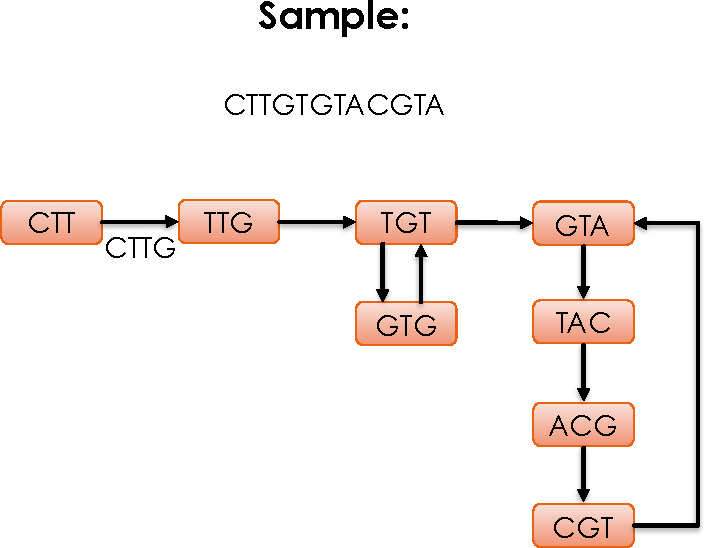
\includegraphics[width=\linewidth]{figs/dbg1-cropped.pdf}
  \caption{de Bruijn graph for a sample with one sequence.}
  \label{fig:dbg-a}
\end{subfigure}%
\begin{subfigure}{.5\textwidth}
  \centering
  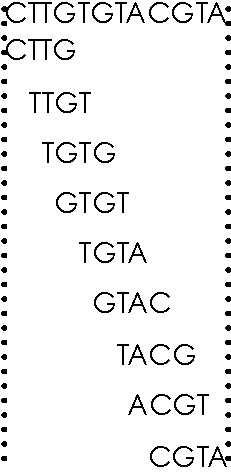
\includegraphics[width=.4\linewidth]{figs/dbg2-cropped.pdf}
  \caption{This example shows how one can reconstruct the reference sequence 
  having a walk through nodes and edges in a de Bruijn graph and taking care of overlaps.}
  \label{fig:dbg-b}
\end{subfigure}
\caption{Building a de Bruijn graph and reconstructing the reference sequence from it}
\label{fig:dbg}
\end{figure}

\dbg is a useful approach for indexing a reference or sequence read because it enables fast querying. One drawback is that for the $k-1$ overlaps between consequent edges, the original data structure is very space-inefficient. For example ABYSS~\cite{simpson2009abyss} represents the \dbg as a hash table with each \kmer as the key and a byte keeping all the connections to other nodes as its value. It needs spending 1 bit to show the existence of each of the edges in forward or reverse-complement case (as we have four characters in our language, we can expand the current node to reach to the next one in at most four different ways in forward direction). The space such a data structure takes is $\abs{E_s}(\frac{k}{4}+1)\frac{1}{\gamma}$ bits where $\gamma \leq 1$, is the hash table loading factor. This storage is considerably large for even one genome data set such as human genome (starting from 40GB while depending on the loading factor can grow to 100GB or more). Yet, a few different data structures and algorithms have been proposed to reduce the size of a \dbg and represent it efficiently. One category of these data structures use Bloom Filter to represent a \dbg~\cite{pell2012scaling,salikhov2013using,chikhi2012space,chikhi2013space,holley2016bloom}. Other than these, there are a few proposed representations that rely on succinct data structures~\cite{gbmp2014sea} and rank and select operations including the original work by Conway and Bromage~\cite{conway2011succinct} and later the work in~\cite{BoweOn12} that is called the BOSS representation of \dbg from the authors’ initials. BOSS is an efficient edge-centric representation of \dbg that takes around 3 bits per \kmer, which is considerably smaller than the hash table representation. This representation provides a complete package for navigation through the \dbg and also an interface to interact and search for a \kmer. In section \ref{sec:rainbowfish}, I explain in more detail, our work on the color representation for a \dbg on top of the BOSS method, using the interface they provide.


\subsection{Compacted de Bruijn Graph}
\label{subsubsec:cdbg}
In addition to all the work that has been done on improving representations for \dbgs, such that a small number of bits are required for each \kmer, there is also a major preparation step in most \dbg preparation pipelines, named compaction. In this step, long paths of \kmers that do not branch are compacted. The process of compacting the \dbg is meant to merge all \kmers in a path in the \dbg with outgoing and incoming degrees less than or equal to one into a single node which is called a \emph{unitig}. The output of this step is called a compacted de Bruijn graph (cdbg), that connects these unitigs and is a variant of the original \dbg with \kmers as nodes. This can be used in the same way as a \dbg for different downstream applications, such as mapping, alignment, variant detection, etc. This method reduces memory by eliminating the great amount of load that overlaps of $k-1$ in consequent \kmers put on memory for cases in the graph that there is only one \textit{possible next} node. For instance, the output node after merging two consequent nodes in a node-centric \dbg with overlap of $k-1$ would be a unitig of length $k+1$ where first base is the first in the source node, the last base is the last in the destination node and the $k-1$ middle bases are shared between source and destination. This compaction step can have a great impact on reducing the memory and is very useful in cases that we are dealing with repeat-heavy sequences~\cite{liu2016debga}. Recently, researchers have designed and implemented algorithms for building a \ccdbg directly from raw data instead of building the memory-inefficient \dbg first and then compacting it in tools such as TwoPaCo~\cite{minkin2016twopaco} and BCalm2~\cite{chikhi2016compacting}. However, indexing a \ccdbg is still a challenge that needs more investigation. 

So far, we know of two other tools, kallisto~\cite{Bray2016Kallisto} and deBGA~\cite{liu2016debga} that are used for indexing \ccdbgs. Although these tools are very efficient in searching for a \kmer, but the memory they need is considerably large so that in case of very large metagenomic datasets their memory exceeds the limits of a moderate server. In section \ref{sec:pufferfish} we propose a memory-efficient indexing data structure for \ccdbgs that has an asymptotically equal \kmer lookup time as the previous tools. we would first use one of the existing tools that we discussed earlier to build the \ccdbg. Later in the same section, we explain our novel data structure to index such \ccdbgs while keeping a balance between space and query time. One great advantage of a specific variant of our indexing structure (sparse indexing) is the flexibility that it provides by giving the option of trading time for space by allowing tunable parameters.

\subsection{Colored de Bruijn Graph}
A \cdbg is a generalized form of a \dbg that allows representing multiple samples in one unified graph while keeping the identity of (and information specific to) each sample~\cite{Iqbal2012Novo}. The samples may be the result of different experiments for the same species, known variants of the same sequence, or metagenomic samples. By counting all of the samples together as one and building a \dbg from them we will lose the variations happening across samples. Colored de Bruijn graphs were originally proposed by Iqbal et. al~\cite{Iqbal2012Novo}  in a tool named \emph{cortex}, useful for variant discovery and genotyping. Each sample is represented with a unique color in a \cdbg and hence all the \kmers coming from that sample will carry that color with them. To be exact, each \kmer or edge in a \cdbg has a color set showing all the samples that this \kmer has appeared in. Maintaining each color separately, we can differentiate between bubbles that are induced by \emph{repeats} when we see the coverage evenly distributed along different paths from \emph{errors} where the error-side has a low coverage~\cite{Iqbal2012Novo}. There are other data structures implemented in tools such as BFT~\cite{holley2016bloom} and VARI~\cite{MuggliBoNo17} for \cdbg. However, in most of the cases specially in VARI and cortex that use BOSS to represent \dbg, color representation is the dominant part in the total space the \cdbg takes compared to a small portion that is taken by BOSS. In section~\ref{sec:rainbowfish} we propose a succinct data structure to represent colors in a \cdbg paired with any \dbg representation that provides a unique index for each \kmer. We theoretically prove and later practically show why our data structure is \emph{succinct} and compare our space and query time results with VARI that uses a similar API to construct the index and find bubbles in \cdbg.


We have other types of graph for representing genomes and transcriptomes such as bidirected graphs \cite{edmonds2003matching,medvedev2009maximum} and biedged graphs that are not the main topics of this document~\cite{paten2017genome}.
%Gcsa?


\section{Genome And Transcriptome Indexing}
\label{subsec:indexing}
Aligning and mapping sequence reads to a reference genome or transcriptome is an important and unavoidable step of many pipelines in genome and transcriptome analysis. For almost all types of quantification and gene/RNA sequence expression analyses, we first need to align short reads to the reference gene/transcript. However, in most of the analyses, this step is the time-consuming bottleneck. To speed up the alignment process, researchers have used different reference sequence indexing methodologies to first find an exact match to a seed from read and continue aligning from that point. With the increasing accumulation of genomic data, there is a need to index massive populations in different research areas. Existing structures for indexing large strings typically fall into two categories; those that are hash-based and provide very fast access to indexed patterns of fixed-length (\kmers)~\cite{liao2013subread} and the linear self indexing methods that are space-frugal and provide asymptotically efficient but practically slower pattern search for arbitrary length patterns, such as Bowtie2~\cite{langmead2012fast} and BWA-MEM~\cite{li2013aligning} that make use of Borrows Wheelers Transform, or suffix array based indices such as STAR~\cite{dobin2013star}. There have been recent efforts to extend both approaches to the context of indexing different types of sequence graphs~\cite{paten2017genome}, with tradeoffs between space and time efficiency. On the succinct self-index side, one notable example is gramtools, the tool in which the graph itself is represented as a modified BWT \cite{maciuca2016natural}. For the recently developed \kmer lookup based approaches, however, it is more prevalent to use graphs as the underlying data structure. The examples are tools like deBGA~\cite{liu2016debga}, genomeMapper~\cite{schneeberger2009simultaneous}, and BGREAT~\cite{limasset2016read}. 

These efforts are interesting, in part, because the \ccdbg, explained in section \ref{subsubsec:cdbg}, has recently emerged as a desirable sequence indexing data structure, because of the efficiency with which it handles repetitive sequences. By definition, any \kmer present in the reference sequence will occur in exactly one \emph{unitig} of the \ccdbg. The absence of duplicate \kmers in the unitig set allows efficient indexing of these \kmers with a minimum perfect hash function (MPHF). In section \ref{sec:pufferfish}, we present pufferfish, an efficient indexing representation of the \ccdbg annotated with information like color, position, orientation, and frequency of each \emph{unitig}. We present two variants of the pufferfish data structure, dense and sparse. The first is optimized for fast queries and the second provides the user with the ability to trade off space for speed in a fine-grained manner.


%\documentclass[a4paper,UKenglish]{lipics-v2016}
%This is a template for producing LIPIcs articles. 
%See lipics-manual.pdf for further information.
%for A4 paper format use option "a4paper", for US-letter use option "letterpaper"
%for british hyphenation rules use option "UKenglish", for american hyphenation rules use option "USenglish"
% for section-numbered lemmas etc., use "numberwithinsect"
 

% Author macros::begin %%%%%%%%%%%%%%%%%%%%%%%%%%%%%%%%%%%%%%%%%%%%%%%%
%\title{\system: A Succinct Colored de Bruijn Graph Representation}
%\titlerunning{\system} %optional, in case that the title is too long; the running title should fit into the top page column

%% Please provide for each author the \author and \affil macro, even when authors have the same affiliation, i.e. for each author there needs to be the  \author and \affil macros
%\author{Fatemeh Almodaresi}
%\author{Prashant Pandey}
%\author{Michael A. Bender}
%\author{Rob Johnson}
%\author{Rob Patro}
%\affil{Stony Brook University, Stony Brook, NY USA\\
%  \texttt{\{falmodaresit,ppandey,rob.patro\}@cs.stonybrook.edu}}
%\authorrunning{Almodaresi et al.} %mandatory. First: Use abbreviated first/middle names. Second (only in severe cases): Use first author plus 'et. al.'

%\Copyright{Fatemeh Almodaresi,Prashant Pandey, Rob Patro}%mandatory, please use full first names. LIPIcs license is "CC-BY";  http://creativecommons.org/licenses/by/3.0/

%\subjclass{``E.1 DATA STRUCTURES'', ``E.2 DATA STORAGE REPRESENTATIONS'', ``E.4 CODING AND INFORMATION THEORY''}% mandatory: Please choose ACM 1998 classifications from http://www.acm.org/about/class/ccs98-html . E.g., cite as "F.1.1 Models of Computation". 
%\keywords{de Bruijn graph, succinct data structures, rank and select operation, colored de Bruijn graph}% mandatory: Please provide 1-5 keywords
% Author macros::end %%%%%%%%%%%%%%%%%%%%%%%%%%%%%%%%%%%%%%%%%%%%%%%%%

%Editor-only macros:: begin (do not touch as author)%%%%%%%%%%%%%%%%%%%%%%%%%%%%%%%%%%
%\EventEditors{}
%\EventNoEds{2}
%\EventLongTitle{}
%\EventShortTitle{}
%\EventAcronym{}
%\EventYear{2017}
%\EventDate{}
%\EventLocation{}
%\EventLogo{}
%\SeriesVolume{}
%\ArticleNo{}
% Editor-only macros::end %%%%%%%%%%%%%%%%%%%%%%%%%%%%%%%%%%%%%%%%%%%%%%%

%\begin{document}
\chapter{\system: A Succinct Colored de Bruijn Graph Representation\protect\footnote{A joint work with Prashant Pandey accepted in WABI2017}}
\label{sec:rainbowfish}
%\maketitle

\section{abstract}
%
  The \cdbg --- a variant of the \dbg which associates each edge (i.e., \kmer)
  with some set of colors --- is an increasingly important combinatorial
  structure in computational biology. Iqbal \etal demonstrated the utility of
  this structure for representing and assembling a collection (population) of
  genomes, and showed how it can be used to accurately detect genetic variants.
  Muggli et al. introduced \vari, a representation of the \cdbg that adopts the
  \boss representation for the \dbg topology and achieves considerable savings
  in space over \texttt{Cortex}, albeit with some sacrifice in speed.  The
  memory-efficient representation of \vari allows the \cdbg to be constructed and
  analyzed for large datasets, beyond what is possible with \texttt{Cortex}.

In this paper, we introduce \system, a succinct representation of the color
information of the \cdbg that reduces the space usage even further. Our
representation also uses \boss to represent the \dbg, but decomposes the color
sets based on an equivalence relation and exploits the inherent skewness in the
distribution of these color sets. The \system representation is compressed based
on the $0$th-order entropy of the color sets, which can lead to a significant
reduction in the space required to store the relevant information for each edge. In practice,
\system achieves up to a $20\times$ improvement in space over \vari. \system is
written in \texttt{C++11} and is available at
\url{https://github.com/COMBINE-lab/rainbowfish}.
%


\section{~Introduction and Related Work}

This paper proposes a new representation of the \cdbg. The \cdbg is a variant of
the \dbg where each edge (i.e., \kmer) is associated with some set of colors.
Here, each color is used to encode the source of the corresponding \kmers (e.g.,
different source genomes, transcriptomes, sequenced samples, etc.). From this
perspective, it is a flexible and powerful combinatorial structure for
representing a collection of sequences while maintaining the identity of each.
This structure gained popularity in the work of Iqbal
\etal~\cite{Iqbal2012Novo}, which demonstrated the utility of the \cdbg for
representing and assembling a collection (population) of genomes, and for
detecting both simple and complex genetic variants with high accuracy. Analysis
of the \cdbg exhibits particular promise for analyzing complex population-level
variation, since topological structures (e.g., bubbles) can be associated with
variation in the underlying sub-populations. The representation adopted by
Iqbal, as implemented in the tool \texttt{Cortex}, is optimized for speed, and
so requires a considerable amount of memory to represent both the topology of
the \dbg and the colors associated with each edge.

The memory usage of the \cdbg representation adopted in \texttt{Cortex}
precludes this approach from being adopted when the underlying genomes and color
sets become too large. In order to overcome such limitations, Muggli et
al.~\cite{MuggliBoNo17} introduced the \vari representation of the \cdbg. This
approach sacrifices some of the speed of the \cortex representation for a
considerable reduction in the required space. \vari achieves this space savings
in two ways.  First, rather than using a hash-table-based representation of the
\dbg topology, it adopts the highly-efficient \boss representation. The
\boss~\cite{BoweOn12} representation (named based on the initials of the
authors) makes use of the FM index~\cite{FerraginaMa00} to encode the topology
of the \dbg. \boss uses $4N + o(N)$ bits to represent a \dbg with $N$ edges
(empirically, this often works out to be as few as 4-6 bits per edge).

\vari couples the \boss representation of the \dbg topology with a compressed
representation of the color information. By its nature, \boss assigns to every
\dbg edge a distinct rank in the range $[0,N)$. So, \vari represents the color
  information as a $N \times C$ bit matrix where $C$ is the number of input colors.
  Conceptually, each of the $N$ rows of this matrix is simply a bit vector that
  encodes which of the $C$ colors label the corresponding edge. To reduce the
  space required to store this color information, \vari concatenates these rows
  into a single vector over $N \times C$ coordinates and stores them in an
  Elias-Fano~\cite{Elias74, Fano71} encoded bit vector, allowing for a
  (sometimes substantial) reduction in the size while still enabling efficient
  point queries (i.e., is a particular edge labeled with a given color?).
  Muggli et al.~\cite{MuggliBoNo17} demonstrate that the \vari representation
  can be built on data sets consisting of large numbers of \kmers, large input
  color sets, or both.  Specifically, the space efficiency of \vari makes it
  possible to build and query the \cdbg on datasets that are orders of magnitude
  larger than what is possible with \cortex.  This is an exciting development
  that opens up this methodology for increasingly large-scale analysis.

  Though \vari achieves a substantial improvement in space over \cortex, there
  is still a considerable amount of redundancy present in its representation.
  Both of these systems represent the color set corresponding to each \kmer
  independently of other \kmers. Hence a considerable amount of redundant
  information can be present when the color set for each \kmer is represented
  independently. In fact, some existing colored de Bruijn Graph representations,
  like the Bloom Filter Trie~\cite{holley2016bloom} exploit this redundancy to
  compress shared color information, and share certain ideas and motivation with
  the representation proposed in this paper. However, many of the possible
  subsets of colors do not occur in practice, and there is an inherent (often
  extreme) skewness in the distribution of the color sets that do appear. It
  becomes even more important to exploit this skewness for large metagenomic
  datasets because the space usage of \vari for these datasets can become
  impractical.

  In this paper, we introduce a succinct representation, called \system, of the
  color sets associated to each edge in the \dbg. We also adopt the \boss
  representation of the \dbg topology, and focus, specifically, on how to
  concisely represent the color information. \system's \cdbg representation is
  entropy compressed and exploits the high skewness present in the distribution
  of color sets. By exploiting a more efficient decomposition of the set of
  present colors (i.e., in terms of equivalence classes), we achieve a
  considerable reduction over the space required by \vari (up to $20\times$
  depending on the dataset), while still retaining efficient (i.e., constant
  time) queries.

%In \system, we construct the color class representation from a color list from
%\vari~\cite{MuggliBoNo17} which in turn uses an efficient representation of
%the \dbg that they call it \boss~\cite{BoweOn12} based on the initials of the
%authors. This representation of \dbg is a generalization of FM indexes that
%can theoretically store a \dbg with m edges in $4m + o(m)$ bits and
%empirically stores \fatemeh{less than 6 bits per \kmer?}. In \boss
%representation we have a CD-lexicographical ordering of \kmers and the support
%for two operations of rank(k) and select(i) over this ordered set. rank(k)
%returns the number of elements before $\kmer_k$ and select(i) returns the
%exact value of \kmer that has $rank=i$. Both \vari and \system consider \kmers
%to be in the same order as returned by rank operation on \boss representation
%of \dbg. \system uses rank-and-select operation to map a \kmer to its color
%class. In the following section we briefly describe the rank and select
%operations. 

\section{~Background and definitions}

\system is a succinct representation of the color information, and uses rank and
select operations to lookup the color class corresponding to \kmers in the \dbg.
Here, we briefly recapitulate the definition of a succinct data structure and the
rank and select operations.

A \defn{succinct data structure} consumes an amount of space that is close to
the information-theoretic optimum. More precisely, if $Z$ denotes the
information-theoretic optimal space usage for a given data structure, then a succinct
data structure uses $Z + o(Z)$ space~\cite{Jacobson89}.

%\rp{this sub-sections seems redundant with the description above}
%\subsection{~\vari 's representation} In \vari the color information is
%stored, conceptually, a an subset from a set of $C$ colors for each of $N$
%\kmers are represented in a color matrix of size $N*C$ bits. If a bit in cell
%$(i, j)$ is set it means \kmer with rank $i$ has color $j$ (i.e. appears in
%$j^{th}$ sample). \vari compresses this uncompressed color matrix using either
%\rrr\cite{} or Elias-Fano\cite{} representation and achieves practical
%compression, but still in worse case scenario the color matrix storage is
%order of $N*C$.

\defn{rank} and \defn{select}~\cite{Jacobson89} are operations that are commonly
used for navigating within succinct data structures. For a bit vector
$B[0,\ldots,n-1]$, \rank$(j)$ returns the number of $1$s in the prefix
$B[0,\ldots,j]$ of $B$. \select$(r)$ returns the position of the $r$th $1$, that
is, the smallest index $j$ such that \rank$(j)=r$. For example, for the 12-bit
vector $B[0,\ldots,11]=$\texttt{100101001010}, \rank$(5)=3$, because there are
three bits set to one in the 6-bit prefix $B[0,\ldots,5]$ of $B$, and
\select$(4)=8$, because $B[8]$ is the fourth $1$ in the bit vector.

\section{~Method}
\label{method}

\begin{figure}[t]
  \centering
  \resizebox{0.70\linewidth}{!}{
    %\ifpdf
      \input{cdbg-rep.pdf_tex}
    %\else
      %\input{cdbg-rep.eps_tex}
    %\fi
    }
  \caption{
    The representation of color information in \system. The ``Color Matrix'' at
    the top represents $6$ distinct $4$-mers, each assigned a color set. $3$ of
    these $4$-mers (ACTG, TTTC, AGCC) have the same color class, labeled $0$,
    and the other $3$ (CTTG, ACTT, and GCGT) each have color classes labeled
    $1$, $10$, and $11$ respectively. To retrieve the color set for a \kmer, we
    first perform select on the boundary bit vector (BBV) using rank $r$ of the
    corresponding edge (\kmer). This returns the label's starting position, $i$.
    We then look for the next set bit BBV to find the label's ending position,
    $j$. Then, we fetch the label at indices $i$ to $j$ in label bit vector
    (LBV). Finally, we lookup the label $l$ in the equivalence class table (ECT)
    and return the color class corresponding to the label. A detailed
    explanation of the data structure and its construction is given in
    \Cref{design}.
  }
    \label{fig:cdbg-rep}
\end{figure}

In this section we first describe the design of \system. We then analyze the
space usage and provide a lower bound for the representation of sets of colors given
a ranking of \dbg edges. Finally, we discuss the \system implementation.

\subsection{~Design}
\label{design}

\system's compact representation of color information is based on two particular
observations. First, it is often the case that many of the \kmers in a \cdbg
share the same set of colors. More formally, we define an equivalence relation
$\sim$ over the set of \kmers in the \dbg. Let $\cfun{\cdot}$ denote the
function that maps each \kmer to its corresponding set of colors. We say that
two \kmers are color-equivalent (i.e., $k_1 \sim k_2$) if and only if
$\cfun{k_1} = \cfun{k_2}$. We will refer to the set of colors shared by the
\kmers related by $\sim$ as a \defn{color class}. If $C$, the number of input
colors, is large, it is often the case that the number of distinct color classes
is far less than the number of possible color classes (which is bounded above by
$\min(N,2^C)$).

Second, it is often the case that the frequency distribution of color classes
is far from uniform.  Hence, it will often be useful to record a frequently
occurring color class using a short description (i.e., a small number of bits)
while reserving larger descriptions for less frequent color classes.

%Put another way, both of these observations can be summarized in
%that we expect $H(X_c)$---the entropy of the color class---to be low (i.e., the
%expected value of the information available in each color class is low or
%order-$0$ entropy).

The design of \system is motivated by the above observations. Instead of storing
the color set for each \kmer separately, \system stores each distinct color
class only once and assigns to each distinct class a label (which, practically,
is much smaller than the unary encoding of the color class itself).
%
%\fatemeh{Furthermore, by replacing the fixed-length label with a variable-length
%one \system leverages the skewness property of distribution of \kmers across
%distinct color sets to save even more space.}
%
%starting from label 0 with 1 bit length. 
%
It then stores, for each \kmer, the label of the color class to which it
belongs. 
%
%Considering the skewed distribution of color class frequencies, this data
%structure can practically be much more efficient compared to the unary encoding
%of the color sets for each \kmer.

The approach we use to assign variable-length labels to color classes is similar
in spirit to the construction of a Huffman code, where the message is a string
of color class symbols. However, we do not build a prefix code, and instead opt
to store an additional bit vector to allow the efficient selection of an
arbitrary label from the list. We generate the labels according to the following
procedure. We first sort, in descending order, all the color classes based on
their frequency (i.e., the number of \kmers in this color equivalence class). We
then assign labels to each color class starting from the class with the largest
cardinality, so that the color class represented by the most frequent label will
have the shortest label length etc.

%The approach we use to assign variable-length labels to color classes is
%similar in spirit to the construction of a Huffman code, where the message is a
%string of distinct color sets (each representing symbol of a color class) and
%frequency of each symbol is frequency of each color class or in other words
%number of distinct \kmers observed with that color set. However, we do not
%build a prefix code, and instead opt to store an additional bit vector to allow
%the efficient selection of an arbitrary label from the list. We generate the
%labels according to the following procedure. We first sort, in descending
%order, all the color classes based on their frequency (i.e., the number of
%\kmers that display this color class). We then assign consecutive numbers as
%labels to each color class starting from the color class displayed by the most
%\kmers, so that the color class appearing as the most frequent label will have
%the shortest label length (which is 1 bit) etc.

The color class representation in \system has three components. \system stores
the mappings between labels and color classes in an \defn{equivalence class
  table (ECT)}. As labels are assigned sequentially, this is simply an array of
bit vectors encoding the corresponding color sets. Apart from the equivalence
class table, \system maintains two bit vectors, a \defn{boundary bit vector
  (BBV)} and a \defn{label bit vector(LBV)}.

All color classes are stored in the equivalence class table (with their
corresponding labels implicitly being their position). However, we now need to
store a mapping from \kmers to the variable-length labels. \system stores
variable-length labels corresponding to each \kmer in the label bit vector. The
labels are stored in the order in which \kmers are stored in the \dbg
representation. Specifically, the \kmers are stored in the rank order induced by
\boss. However, since these labels are variable-length, we can not directly read
the label corresponding to the \kmer of a specific rank, since we do not know
where such a label begins or how long it is.

To address this, \system maintains another bit vector --- the boundary bit
vector (BBV) --- to mark the boundary of each variable-length label in LBV. The
BBV is the same size as the LBV and has a bit set
to 1 at each index where a new label starts in the LBV. Thus, the starting
position for the label corresponding to the $r$th \kmer can be obtained by
issuing a \select{(r)} query on BBV, and the length of this label can be
obtained by simply scanning BBV until we encounter the next set bit.

\Cref{fig:cdbg-rep} shows how the color classes are represented in \system. To
perform a query for the color class corresponding to a \kmer in the \cdbg, we
first get the rank $r$ of the \kmer in the \dbg. We then perform a select
operation using $r$ on BBV. The result of the select operation $i$ is the start
index of the label of the color class in LBV to which the \kmer belongs.
%
To find the length of the label we determine the index $i'$ of the next bit set
in BBV using the \textsc{tzcnt} instruction.
%
\textsc{tzcnt} returns the number of trailing zeros in its argument. If $B$ is a
12-bit vector such that $B[0,11]=$\texttt{110010100000} then
$\textsc{tzcnt}(B)=5$.
%
%another select operation \fatemeh{we don't do that anymore} using $r+1$ to find
%the start of the next label. The difference between the start of the next label
%$i'$ and $i$ is the length of the label in the label bit vector. 
%
Using $i$ and $i'$ we retrieve the label from LBV, and using
the label we lookup the corresponding color class in ECT.
%
We also note that, as we never have $> 2^{64}$ distinct \kmers in practice, and
number of distinct labels is at max equal to the number of distinct \kmers (when
each \kmer has a unique label), then we never have $> 2^{64}$ labels. Hence, we can
always represent a label using a single machine word. Consequently, we will
always reach the next set bit in the LBV after scanning at most a single machine
word when starting from current label. This ensures we need only issue a single
\textsc{tzcnt} instruction per label decoding call.


\subsection{~Space analysis}
\label{system-space-bound}

The color class representation in \system is entropy compressed, i.e.,
the space is bounded by the entropy ($H(X_c)$) of the color class distribution. 
For a dataset in which number of \kmers belonging to each distinct color class are
similar, the entropy of the color class distribution will be high. On the other
hand, if most of the \kmers in a dataset belong to a small number of distinct
color classes, the entropy of the color class distribution will be low.

\begin{lemma}
  The size of each color class label is bounded by $\log_2{M}$ bits, where
  $M$ is the total number of distinct color classes. For a dataset with $N$
  distinct \kmers coming from $C$ input samples (i.e., colors), we have that $M
  \leq \min(N,2^C)$.
  \label{label-size-bound}
\end{lemma}

%\prashant{I have changed the wording in theorem 1. I don't know if it's better or worse.}

\begin{theorem}
Given an ordering of edges (or \kmers) in a \dbg, the space needed by \system to
represent a set of colors attached to each edge is $\order{MC+N H(X_c)}$ bits,
where $M$ is the number of distinct color classes, $C$ is the number of colors,
$N$ is the number of distinct \kmers, and $H(X_c) = -\sum_{i=1}^{M} P(x_i)\log
P(x_i)$ is the entropy (i.e., order-$0$ or Shannon's entropy) over random
variable $X_c$, which distributed according to the frequency distribution of the
color classes.
%$H(X_c)$ is the entropy of the color class distribution. 
\label{space-bound} \end{theorem}

\begin{proof}
%
The space needed by \system can be analyzed as follows. There are three bit
vectors in \system, the equivalence class table, label bit vector, and boundary bit
vector. To store an equivalence class table containing $M$ distinct color
classes each having $C$ colors we need $MC$ bits. To store a label bit vector
(as stated in \Cref{label-size-bound}), for $N$ \kmers, where each label
corresponds to one of the $M$ distinct color classes, takes $N\log_2{M}$ bits.
However, as explained in \Cref{design}, in \system we assign (optimal) variable-length
labels based on the frequency of color classes. Therefore, the space needed to
store the label bit vector is dependent on the $0$th-order entropy of the color
class variable, $H(X_c)$, and the size of the label bit vector is upper bounded
by $N\log_2{M}$.  The boundary bit vector has the same number of bits as the
label bit vector. 
%
\end{proof}

%%
% This seems redundant
%%
%As explained in \Cref{space-bound}, the space required to represent the label
%bit vector in \system depends on the entropy of the color class distribution.
%For a uniformly-random distribution the space would be high compared to a skewed
%distribution. The boundary bit vector contains the same number of bits as the
%label bit vector.


\subsection{~Lower bound for color representation}

%\fatemeh{I think we need a few sentences here to say we divide the space bound
  %to equivalence table space and label/boundary bit vectors and explain we are
  %already succinct regarding storing the equivalence table with space bound of
  %$\order{MC}$. Then say we now prove why we are also succinct regarding
  %label/boundary bit vectors with practical space of $\order{NH(X_c)}$}

We now provide a lower bound to store a color class representation for a set of
edges in a \cdbg. In the color class representation, the equivalence class table
takes $MC$ bits to store $M$ bit vectors each having $C$ bits, which is
optimal. The other two bit vectors, the boundary and label bit vector, map \kmers
given an ordering in the \dbg to their corresponding color classes. The theorem
below gives the lower bound to store such a mapping.
 
\begin{theorem}
%
  The lower bound to represent a mapping from an ordered list of \kmers in a
  \dbg to a set of color classes is $\log_2{(M^{N-M} \cdot M!)}$ bits, where
  $M$ is the number of distinct color classes, $N$ is the number of edges, and
  for a dataset with $N$ distinct \kmers coming from $C$ input samples (i.e.,
  colors), we have that $M \leq \min(N,2^C)$.
%
\end{theorem}

\begin{proof}

We can analyze the lower bound using a counting argument. We count the number
of ways to map a set of $M$ distinct color classes to a set of $N$ edges. The
space required to store the color class representation should be less than or
equal to the space required to store these mappings.

Edges can be mapped to color classes using a surjective (onto) function. Thus,
we wish to count the total number of surjections from $M$ color classes to $N$
edges. Rather than counting this number exactly, we instead provide a lower bound.
First, we must ensure that each of the $M$ color classes maps to at least one
edge --- so, we select a set of $M$ edges and label each with a distinct color
class. There are $M!$ ways to assign $M$ color classes to a set of $M$ edges. We
will then allow the remaining $N-M$ edges to be colored in any possible manner.
We can assign $M$ colors to $N-M$ edges (the remaining number) in $M^{N-M}$
ways. Therefore, the total number of different mappings is bounded below by $M^{N-M}
\cdot M!$. To be able to represent each such mapping, and distinguish it from
the others, we need at least $\log_2{(M^{N-M} \cdot M!)}$ bits.
\end{proof}

The lower bound can be expanded using Sterling's approximation as
\[
(N-M)\log_2{M} + M\log_2{M} - 0.44M + O(\log_2{M}),
\]
which, ignoring the
additive term $\order{\log_2{M}}$, is greater or equal to $N\log_2{M} - 0.44M$. Given the range of
$M$ (i.e., $1 \leq M \leq N$), $N\log_2{M}$ always dominates the lower bound.

Now, we show that the space needed by \system to store the variable-length
labels assigned to color classes is equal to the lower bound. As explained in
\Cref{label-size-bound}, the upper bound to store any label is $\log_2{M}$ bits,
and for $N$ edges, it is given by $N\log_2{M}$ bits.  \system also stores a
boundary bit vector which has the same number of bits as the label bit vector.
Therefore, the space required to store the label mappings is strictly $\leq
2N\log_2{M}$. Note that the extra overhead to store the metadata to perform a
select operation in constant time on the boundary bit vector is bounded by
$o(N)$, where $N$ is the numbers of bits in the bit
vector~\cite{GonzalezGrMa05}.

However, \system's representation of color classes is entropy compressed (see
\Cref{design}) and the space required depends on the entropy of the color class
distribution. For a highly skewed distribution, the entropy is low and the space
required to store labels is much smaller than $N\log_2{M}$ bits. On the other
hand, when the distribution is near-uniform, i.e., the entropy is high, \system
makes all labels to be $\log_2{M}$ bits and dispenses with BBV. Therefore, the
space required by \system is always smaller than or equal to the lower bound.

%\fatemeh{Here we are proving ds <= O(Z) while for succinct we should prove ds
%= Z + o(Z). The first is the proof for compact. So one idea we discussed with
%Robp is to remove $\order{}$ from $\order{N\log_2{M} -/+ blabla}$ and consider
%it as $Z'$ which is itself a lower bound on Z ($Z' = Z + o(Z)$). Then we prove
%ds = $Z' + o(Z') = Z + o(Z) + o(Z + o(Z)) = Z + o(Z)$}


\subsection{~Implementation}

\tikzsetnextfilename{plant-eq-class-dist}
\begin{figure}[h]
\centering
\begin{tikzpicture}[scale=0.8]
  \begin{axis}[
    ybar,
    %x=2pt,
    %height=6cm,
    bar width=3pt,
    xtick=data,
    scaled ticks=false,
    ymode=log,
    ymin=0,
    ylabel={\#\kmers in each equivalence class},
    xlabel={Equivalence class labels},
    legend style={at={(1.05,0.63)}, anchor=north west},
    nodes near coords align={vertical},
  ]
    \pgfplotstableread{data/plant-eqDist-1pass}\loadedtable;

      \addplot[color=teal, fill=teal] table[x=x_0, y=y_0] {\loadedtable};
      \addplot[color=olive, fill=olive] table[x=x_0, y=y_1] {\loadedtable};
      %\addplot[color=teal, fill=teal] table[x=x_0, y=y_2] {\loadedtable};
      \legend{Color class dist. in $1$-pass,Color class dist. in $2$-pass}
    \end{axis}
\end{tikzpicture}
    \caption{
    Distribution of \kmer frequencies across equivalence class labels in \system
    after $1$-pass and $2$-pass algorithm on plant dataset
    \Cref{tab:datasets-info}. The $2$-pass algorithm assigns the smallest label
    to color class with maximum number of \kmers. The distribution in $2$-pass
    algorithm is monotonically decreasing. 
  }
      \label{fig:plant-eq-class-dist}
\end{figure}

\subparagraph{Considerations due to the underlying \dbg representation} We recall here that we make use of the BOSS representation of the underlying \dbg topology. To build the BOSS representation, \kmer counting is first performed using KMC2~\cite{Deorowicz15KMC}, canonicalizing \kmers during counting. Though the BOSS representation inserts both forward and reverse complement \kmers into the graph, it associates only a single color vector with this pair.  Moreover, BOSS creates ``dummy'' edges (real \kmers prepended or appended with \$) to allow encoding \kmers that appear near terminal nodes in the \dbg. In the \cdbg these dummy edges are assigned the empty color set. All of this information is encoded by both \vari and \system. However, as we discuss in more detail in~\Cref{sec:conclusion}, the \system representation can work with any \dbg representation that can assign distinct ranks to each \kmer in the \dbg. Thus, we would expect this encoding scheme to work well with, e.g., a \dbg representation based on minimum perfect hashing of the
\kmers~\cite{drezen2014gatb}.
%\fatemeh{We should note that as BOSS counts a \kmer and its reverse complement as two distinct \kmers, we also count them as two different \kmers.}

\subparagraph{Storing bit vectors.} In \system, we use bit vector implementations
from the SDSL library~\cite{sdsl} to store the three bit vectors from
\Cref{fig:cdbg-rep}. We use the $rrr\_vector$ implementation from SDSL to store
the equivalence class table and boundary bit vector, and the $bit\_vector$ implementation
from SDSL to store the label bit vector.

The $rrr\_vector$ of SDSL is an implementation of \rrr encoding~\cite{RamanRaRa02}. \rrr
encoding is an entropy compressed encoding and also supports constant time rank
and select operations on the compressed bit vector.  The space reduction depends
on the entropy of the bit vector. For high entropy bit vectors, the compression
is not noticeable and in fact ``negative'' in some cases because of the extra
metadata overhead to support rank and select operations.

The equivalence class table and boundary bit vector often have fairly low
entropy, and can be compressed efficiently using RRR encoding. However, the
label bit vector often has high entropy, and compressing it using \rrr encoding
is not effective. In our representation, the average order-$0$ entropy of the
label bit vector for four different datasets is $0.94$. This is a quite high,
and hence we did not see any reduction in the space using \rrr encoding.
However, for the other two bit vectors, the order-$0$ entropy is lower (e.g.,
for boundary bit vector the average entropy over same four datasets is $0.56$)
and, in practice, we achieve a considerable space reduction using RRR encoding.

\subparagraph{Construction.} We use a $2$-pass algorithm to construct the three bit vectors. In the first pass, we read the color matrix, compute the distinct color classes, and count the frequency of each class. Once we have the frequency information, we sort color
classes in descending order based on their frequency. We then assign labels to
color classes starting from zero. In the second pass, we read the uncompressed
color matrix again, and add the label of each \kmer to the label bit vector.
While building the label bit vector, we also build the boundary bit vector by
storing a $1$ at every index where a new label starts in the label bit vector.
The labels are stored in the same order as the \kmers in the \boss
representation.

To reduce the space required for the labeling even further, we implemented our label
encoding in the following way. Every time that the label size increases from $x$
bits to $x+1$ bits, we restart the counter of that label in label bit vector to
$0$. For example, we store $0$ and $1$ for labels $0$ and $1$ respectively,
then we store $00$, $01$, $10$ and $11$ for labels $2$, $3$, $4$ and $5$
respectively. For label value $6$ we again restart the counter to $0$ and store
$000$ to represent $6$ in the label bit vector, etc. Later, when we want to retrieve
the actual value of a label, we first recover the stored label $l'$ from the label
bit vector and then calculate the actual label $l$ using the equation $l = l'
+ 2^{d}-2$ where d is length of label $l$ in bits.

As explained in \Cref{system-space-bound}, the $2$-pass algorithm minimizes the
space used to represent color class labels by sorting the classes based on their
frequencies and assigning labels to color classes to minimize the length of the
resulting code path, similar to Huffman coding. However, one could also imagine
assigning labels to color classes as we see them in the order \kmers appear in
the \boss representation. This way, we can construct all three tables in a single
pass (i.e., a $1$-pass algorithm).

However, as shown in \Cref{fig:plant-eq-class-dist}, this $1$-pass algorithm can
end up assigning long labels to frequent \kmers, and hence produce poor (i.e.,
large) encodings. However, the $2$-pass algorithm always assigns labels
according to the corresponding frequency distribution of the color classes.
Sometimes, the $1$-pass algorithm does well, but we chose to adopt the $2$-pass algorithm
in \system. 

\section{~Evaluation}

\begin{table}
  \begin{center}
    \begin{tabular} {| l | c c c|}
    \hline
      Datasets & \# of edges & \# of colors (samples) & \# of distinct color classes \\
      \hline
      \ecoli 10 & 28,273,951 & 10 & 479\\
      \ecoli 1000 & 157,737,064 & 1000 & 2,669,157 \\
      \ecoli 5598 & 435,705,390 & 5598 & 7,000,715\\
      \ecoli 1000 (k=63) & 258,893,268 & 1000 & 2,530,253\\
      Plant & 2,520,140,426 & 4 & 16 \\
      Beef safety & 97,096,576,010* & 87 & 623,022,532\\
      Human transcriptome & 159,441,804* & 95,146 & 340,762\\
      \hline
      % &  e-coli 10 & e-coli 1000 & e-coli 5598 & Plant & Beef Safety \\
      %Num. of Edges &  & 157,737,064 & 435,705,390 & 2,279,614,458 & \\
      %Num. of Colors & 10 & 1000 & 5598 & 4 & 87 \\
    \end{tabular}
  \caption{
    The number of edges (include \kmers and dummy edges in the BOSS
    representation), samples and color classes for different datasets used in
    the experiments. $k = 32$ unless otherwise specified. \small
    *\# of edges excluding dummies.
}
\vspace{-2.5em}
  \label{tab:datasets-info}
\end{center}
\end{table}

\begin{table}
\begin{center}
\begin{tabular} {| l | c c| c c|}
\hline
Datasets & \multicolumn{2}{c|}{Construction Time (secs)} & \multicolumn{2}{c|}{Bubble Calling Time (secs)} \\
\cline{2-5}
& \vari & \system & \vari & \system \\
\hline
\ecoli 10 & 44 & 31 & 344 & 366\\
\ecoli 1000 & 340 & 270 & 2,610 & 2,356\\
\ecoli 5598 & 3,141 & 4,021 & 8,796 & 8,201\\
%\ecoli 1000 (k=63) & 323 & 257 & 3,971 & 7,546\\
\plant & 108 & 339 & 47,040 & 48,537\\
\beefsafety & 15,378 &  30,478 & NA & NA\\
Human transcriptome & 13,961 & 30,804 & NA & NA\\
\hline
\end{tabular}
\caption{
  Construction and bubble calling time for \system and \vari for different
  datasets. 
}
\vspace{-2.5em}
\label{tab:time}
\end{center}
\end{table}

In this section we evaluate \system, and compare it to \vari~\cite{Muggli17}, a
state-of-the-art \cdbg representation. We evaluate both systems in terms of
space and running time. We address the following questions about the performance
of \system: How does \system compare to \vari in terms of the space required to
represent color information?; How does \system compare to \vari in terms of the
construction time?; How does \system compare to \vari in terms of typical
queries (e.g., in bubble calling)? We are particularly concerned with ensuring
that \system produces small encodings of the color information and remains
practically efficient to query.

\subsection{~Experimental setup}

To answer the above questions, we perform two different benchmarks. First, we
evaluate the time taken to construct the color class representation. The
construction time is the time taken to construct the color class representation
from a list of color classes stored in the order of the edges in the \dbg (this
is the same input used by \vari). During construction, we adopt a two-pass
algorithm. In the first pass, we use a sparse hash-table to determine the distinct
color classes and the cardinality of each such class.

We note that the space taken in this first pass is within a small constant
factor of the final space required by the final ECT table itself, since we need
only store each color class once in the hash table (as a key), and store the
associated count (a machine word) as the value.  Thus, the memory required by
this first pass is almost always a small fraction of the total memory usage 
of the construction algorithm.

Given this information, we know exactly the number of bits that will be required
to store the label and boundary vectors. In the second pass, we fill in both the
label and boundary vectors and then save all three structures to file. As with
most succinct representations, the space required for our data structure in
memory and on disk is almost the same (as the two-pass algorithm allows us to
allocate only the space we need for our final representation). The construction
time recorded here does not include (for either \system or \vari) the time taken
to build the \dbg and color list corresponding to edges in the \dbg (since this
is the same for both methods).

We also report the space needed by both \system and \vari to store the color class
representation on disk. We do not include the space needed to represent the
actual \dbg in our space comparisons because both \system and \vari use \boss
to store the actual \dbg, and the \boss representation itself tends to take less
space than the color information.

Second, we evaluate the time taken to perform the bubble calling benchmark as
described in~\cite{MuggliBoNo17}, using both the \vari and \system
representations. Finding bubbles in a \cdbg enables one to detect regions in the
\dbg where different samples (i.e., colors) diverge from each other. As
originally suggested by Iqbal et al.~\cite{Iqbal2012Novo}, such algorithms can
form the basis for analyzing certain types of genetic variants in populations of
genomes. We note that we adopt the exact bubble calling algorithm implemented in
\vari, and the only variable being altered in our bubble-calling benchmark is
the data structure being used to determine the set of colors present for each
\kmer. Since \vari and \system are both built upon the \boss representation,
which is based on the edge-centric view of \dbg, they consider \kmers as edges
in the \dbg, meaning that each edge is associated with a \kmer, and its
corresponding rank and color set. Briefly, the bubble calling algorithm takes as
input a pair $c_1,c_2$ of colors and traverses edges in the \dbg to find bubbles
in which the edges in one sub-path are colored with $c_1$ and the edges in the
other sub-path are colored with $c_2$ (see~\cite{MuggliBoNo17} for further
details).

For all experiments in this paper, unless otherwise noted, we consider the \kmer
size to be $32$ to match the parameters adopted by Muggli et
al.~\cite{MuggliBoNo17}. We carry out these benchmarks on a number of datasets
as described in \cref{subsec:data}. The time reported for construction and
bubble calling are averaged over two runs, and the time is measured as the
wall-clock time using the \texttt{/usr/bin/time} executable. All experiments
were performed on an Intel(R) Xeon(R) CPU (E5-2699 v4 @2.20GHz with 44 cores and
56MB L3 cache) with 512GB RAM and a 4TB TOSHIBA MG03ACA4 ATA HDD running ubuntu
16.10, and were carried out using a single thread. We note that, while the
construction of the color set representation in \system (and \vari) are serial
operations, queries are trivially parallelizable, as each label can be queried
and decoded independently.

\subsection{~Data}
\label{subsec:data}

We run our benchmarks on the datasets mentioned in \Cref{tab:datasets-info}.
The first three datasets, 
%All three datasets 
\ecoli, \plant, and \beefsafety are slight variants of those used for
evaluation in \vari~\cite{MuggliBoNo17}. Each of these data sets exhibits
different characteristics in terms of the number of \kmers, the number of input
samples (i.e., colors) and the homogeneity of the underlying samples (i.e., how
different are the \dbg for each of the individual samples).
%
The first dataset consists of the assemblies of 5,598 different strains of
\ecoli obtained from GenBank~\cite{o2015reference}. Here, each ``color''
represents a specific \ecoli assembly. Since these assemblies are from
different strains of the same species, they exhibit a small degree of
heterogeneity. In other words, a large fraction of the union \dbg is expected
to occur in all samples.

To evaluate the scalability of \system when primarily changing the underlying
number of input colors, we have evaluated three variants of the \ecoli dataset.
These consist of a dataset containing only 10 different strains, another
containing 1,000 different strains and the final containing all 5,598 strains.
We also performed experiments with \kmer size to be $63$ for \ecoli 1000
dataset to evaluate the space usage for higher \kmer sizes.


%All these experiments are conducted on set of \kmers derived from
%the data with $k=32$. In addition to that, to evaluate the effect of k in for
%\kmers in the space required by \system we ran it \kmers with $k=63$ from
%\ecoli 1000.

%Using all \ecoli assembly samples we will have \kmers from 5,598 different
%colors. To evaluate the effect of varying number of colors on storage and
%performance of \system, we design three different experiments on \ecoli data
%running all steps of the process on the first 10, 1000, and then all 5,589
%\ecoli samples. 
The second dataset (i.e., \plant) consists of the genome assemblies of four
different plant species. Hence, this dataset contains only four colors, but has
more than $\approx2$ billion distinct \kmers. The plant species considered are,
\fnurl{\textit{A}. \textit{thaliana}
}{ftp://ftp.ensemblgenomes.org/pub/plants/release-34/fasta/arabidopsis_thaliana/dna/Arabidopsis_thaliana.TAIR10.dna.toplevel.fa.gz}~\cite{swarbreck2008arabidopsis},
\fnurl{Corn}{ftp://ftp.ncbi.nlm.nih.gov/genomes/all/GCF/000/005/005/GCF_000005005.1_B73_RefGen_v3/GCF_000005005.1_B73_RefGen_v3_genomic.fna.gz}~\cite{schnable2009b73},
\fnurl{Rice}{http://rice.plantbiology.msu.edu/pub/data/Eukaryotic_Projects/o_sativa/annotation_dbs/pseudomolecules/version_7.0/all.dir/all.con}~\cite{tanaka2008rice},
and
\fnurl{Tomato}{ftp://ftp.solgenomics.net/tomato_genome/assembly/build_2.50/SL2.50ch00.fa.tar.gz}~\cite{causse2013whole}.
%
These genomes exhibit considerable diversity and heterogeneity. Given the
diverse regions in the \cdbg, this dataset is a good candidate for the bubble
calling benchmark. Further, Muggli et al.~\cite{MuggliBoNo17} found that this
was the only of the three original datasets on which they were able to construct
the original \texttt{Cortex} representation of the \cdbg. They validated
\texttt{Cortex} produces the same bubble calls as \vari ~\cite{MuggliBoNo17}
(which, of course, produces the same bubble calls as \system).
%
For more detailed analysis of \texttt{Cortex}'s construction and processing time
and space on this dataset, please refer to~\cite{MuggliBoNo17}.
%
%among different samples that later will be critical for time evaluation in
%bubble finding process as there will be a lot of branching in \dBG and hence a
%lot of access queries for pair of \kmer and color on each branch. 
%

The third dataset, \beefsafety, is considerably different from the prior data.
Instead of the input samples consisting of assembled genomes, they consist of
87 metagenomic samples sequenced from cattle in the commercial process of beef
production~\cite{noyes2016resistome}. Hence, this dataset yields a considerably
larger and more complex \dbg since it is built upon many un-assembled (and
non-error-corrected) reads. Thus, the \dbg will encode portions of the relevant
metagenomes as well as the effects of sequencing errors. This dataset also has
many more \kmers than the others, $\approx97$ billion. It exhibits a large
degree of heterogeneity and an intermediate number of input colors (87).
%
%is a doubly huge dataset with total amount of 97,096,576,010 \kmers and
%considerable number of colors (87) and heterogeneity which provides a good
%practical example to evaluate time and space of \system compared to
%state-of-the-art colored \dBGs, \vari. 
%

In addition to the three datasets used in the \vari paper, we also consider
building the \cdbg on the \fnurl{human
transcriptome}{ftp://ftp.sanger.ac.uk/pub/gencode/Gencode_human/release_26/gencode.v26.pc_transcripts.fa.gz}
(Gencode v26 protein coding transcripts)~\cite{Harrow2012}. Here, we consider
each transcript as an individual sample (i.e., a distinct input color). This
data consists of $\approx95,000$ colors, but only $\approx159$ million \kmers.
Hence, this dataset will give an idea about how the representations
will perform when the number of colors becomes very large (though the number of
distinct color classes remains orders of magnitude smaller than the number of
\kmers). Further, we note that this dataset highlights some of the similarities
between the color class encoding adopted by \system and the \kmer-based
equivalence class decomposition adopted by certain transcript quantification
methods (e.g.~\cite{PatroSailfish:2014}).

%The fourth dataset illustrates another use case for \cdbg tools other than
%metagenomic analysis. This dataset is human transcriptome in which we consider
%each transcript as an individual sample, so that the \cdbg built upon this
%dataset has as many colors as transcripts.

%\footnote{ftp://ftp.ensemblgenomes.org/pub/plants/release-34/fasta/arabidopsis_thaliana/dna/Arabidopsis_thaliana.TAIR10.dna.toplevel.fa.gz}
%,
%\fnurl{Corn}{ftp://ftp.ncbi.nlm.nih.gov/genomes/all/GCF/000/005/005/GCF_000005005.1_B73_RefGen_v3/GCF_000005005.1_B73_RefGen_v3_genomic.fna.gz},
%Rice
%\footnote{http://rice.plantbiology.msu.edu/pub/data/Eukaryotic_Projects/o_sativa/annotation_dbs/pseudomolecules/version_7.0/all.dir/all.con}
%and Tomato \footnote{
%ftp://ftp.solgenomics.net/tomato_genome/assembly/build_2.50/SL2.50ch00.fa.tar.gz}

\subsection{~Performance}

\Cref{tab:time} shows the time taken by \system and \vari to construct the color
class representation for different datasets. \system uses a $2$-pass algorithm
to construct the color class representation, and hence the construction time is
dominated by the steps to read the color list file twice. For small datasets
like \ecoli $10$ and \ecoli $1,000$, the input file size is small and does not affect
the overall construction time compared to \vari. However, for large datasets
like \plant and \beefsafety, the time to read the color file twice dominates the
construction time and \system is $1.9\times$---$3\times$ slower. We note that
this time can be considerably reduced by avoiding the uncompressed color matrix
representation currently used upstream of \system and \vari, and integrating
determination and encoding of the color classes into the \dbg construction
directly. However, this is outside the scope of the current paper.

\paragraph*{~Space}\Cref{tab:space} shows the space usage of \system and \vari
for the different datasets we consider. Among these data, there are a range of
characteristics in terms of the number of \kmers, the number of colors, and the
complexity and heterogeneity of the \dbg. We find that, for all datasets,
\system requires less space to store the color information than \vari.  The
magnitude of the improvement depends on the number of distinct equivalence
classes and their distribution, but is as large as $\sim 20\times$.  We see the
same trend with higher values of \kmer sizes.

%\fatemeh{Even changing $k$ to higher value doesn't change the trend.}

In particular, \system's space usage is particularly impressive for datasets
with a large number of input colors but a relatively small number of distinct
\kmers. In this case, we usually find that the number of distinct color classes
is very small compared to the universe of possibilities, and so each label can
be encoded in much fewer than $C$ bits. However, the space \vari consumes
depends greatly on the sparsity of the color matrix. The color matrix itself
grows rapidly as the number of \kmers and colors increases, but \vari's
compression mechanism (Elias-Fano encoding) is very effective if the color
matrix is sparse (e.g., each \kmer is labeled with only a small subset of
colors). This is exactly the case for the Human transcriptome, where the color
matrix has an entropy of $\sim 0.0004$ (compared to \ecoli 5,598 and \ecoli
1,000 with entropies of $\sim 0.16$ and $\sim 0.34$ respectively). Thus, in the
\ecoli dataset, \vari can save space up to a factor of $\sim 5$ compared with
the uncompressed representation, while in the Human transcriptome it can save a
factor of $\sim 2,150$ because of the low entropy of the color matrix. \system
does well in all experiments, even when the number of input colors is small
(e.g., in the \plant dataset). \system achieves the most impressive compression
when the color class distribution has low entropy and the number of color classes
is small relative to the upper bound.
In such cases, the entropy compressed representation of \system is able to
represent a large fraction of all labels using a very small number of bits.
%\fatemeh{
%while because of high entropy in color matrix, \vari's space increases as a result of negative compression. 
% --> This low entropy in color class distribution and high entropy in color matrix might be a little bit confusing but really interesting to talk about.} 


\begin{table}
\begin{center}
\begin{tabular} {| l | c c c|}
\hline
Datasets & 
uncompressed color matrix & \vari & \system \\
\hline
\ecoli 10 & 34 & 58 & 20 \\
\ecoli 1000 & 18,804 & 8,848 & 475 \\
\ecoli 5598 & 290,761 & 58,718 & 2,938 \\
\ecoli 1000 (k=63) & 185,669 & 8,872 & 637\\
\plant & 1,202 & 1,603 & 497 \\
\beefsafety & 1,007,009 & 210,998 & 144,564 \\
Human transcriptome & 1,808,435 & 841 & 817 \\
\hline
\end{tabular}
\caption{
  The space required by \system and \vari to store the color class
  representation for different datasets. The first column shows space required for the uncompressed color matrix ($N \times C$ bits).
  All space is reported in MB. $k = 32$ unless otherwise specified.
}
\vspace{-3.5em}
\label{tab:space}
\end{center}
\end{table}

%Based on the design of our data structure we would expect to see an order of
%magnitude improvement in storage as number of colors increase. We expect to do
%as well as \vari in case of 10 samples of \ecoli as a small dataset with few
%colors and do much better regarding space in case of considering all 5,598
%samples. table \ref{tb:space} shows changes of storage while changing number
%of colors. As shown in table \cref{tb:space} \system improves space when
%number of colors increase from taking 16 times less space in \ecoli with 1000
%samples to 26 times in full \ecoli dataset compared to \vari. 

%Another interesting result is the huge amount of space improvement we see in
%\plant dataset although it has just four colors which implies that \system not
%only works better in terms of increasing number of colors but also when we have
%a huge amount of \kmers. While in \vari, they keep four bits per each \kmer in
%\plant dataset (one bit for each color and hence four bits for four colors),
%but still replacing that with two bits for the first two most frequent color
%sets in \system can still save a lot of space when we have a considerable
%amount of \kmers even with the overload of saving equivalence table.

\paragraph*{~Bubble calling} \Cref{tab:time} shows the time taken by \system and \vari to perform the bubble
calling benchmark on different datasets. We run the bubble calling benchmark on
the \ecoli and \plant datasets (as in the \vari paper). We note that the current
bubble calling algorithm is too slow to run on the Beef safety data set (the
time in~\cite{MuggliBoNo17} was estimated at $>3,000$ hours). It is possible,
however, that optimizations to the underlying algorithm might lift this
restriction. We also did not perform bubble calling on the human transcriptome
dataset as here, we were unable, given the resources on our server, to even run
the \dbg construction to completion. Specifically, due to the large amount of
external memory that \vari uses to build the uncompressed color matrix and the
\dbg on these larger (either in terms of the number of \kmers, the number of
colors, or both) datasets (on order of Terabytes), we exhausted the available
disk space. For these datasets, to approximate the relevant sizes and
construction times, we produced a uncompressed color matrix that lists the
colors for each \kmer and its reverse complement, and we use this to build both
the \vari and \system color representations. While very similar to the full color
matrix that \vari would produce, this file is slightly different in that it does
not include entries for dummy edges (a detail of the \boss representation), and
the order of the color matrix rows can be different from what will appear in the
\boss representation. However, we still believe these numbers, provided in
\Cref{tab:datasets-info}, give a reasonable approximation of how the respective
methods would perform were we able to construct the \dbg completely.

For bubble calling, both representations require a very similar amount of time.
This is likely due, in part, to the fact that navigating the \boss
representation of the \dbg may be the performance bottleneck in the bubble
calling algorithm. Thus, both \vari and \system provide sufficiently fast access
to the color sets for each edge that they do not represent bottlenecks in this
regard.

\section{~Conclusion and Future Work}
\label{sec:conclusion}

In this paper, we propose an entropy-compressed, succinct data structure to
store the color information of a \cdbg. To represent the topology of the \dbg
itself, we adopt the \boss~\cite{BoweOn12} representation. However, we note
that, for our representation of the color sets, we only require that the
underlying \dbg representation is able to associate a unique rank between $0$
and $N-1$ with each edge. Hence, it is possible to use the \system
representation with other representations of the \dbg topology (e.g., those
based on minimal perfect hashing).

We demonstrate that the inherent skewness in the distribution of color classes
can be exploited to reduce the size of the color information. This allows
\system to represent the \cdbg, even for large datasets with many colors, in a
reasonably small space. In fact, for representing the color information itself,
we show that \system is succinct, and hence requires only $Z + o(z)$ bits where
$Z$ is the number of bits required by an information-theoretically optimal
representation.
%
Moreover, it may be possible for the color information stored in the equivalence
class table to be further compressed to reduce the space. For example, one could
imagine an encoding of color sets that takes advantage of their shared subsets,
e.g., storing the shared prefixes of membership vectors only once.
%
%It's also likely that reordering \kmers would reduce the entropy of the label
%vector and result in higher compression ratio. For example, \kmers appearing
%nearby in the \dbg have a higher probability of having the same color class.
%Reordering \kmers based on the \dbg traversal order can bring \kmers with same
%equivalence classes together and thereby increasing the skewness in the color
%information.

%\fatemeh{We keep each color once in ECT and later refer to that with its
%corresponding label for each \kmer and we prove that this representation is
%indeed succinct. However, we can still push compacting color representation in
%ECT even one step further to improve $o(z)$. For example we can exploit the
%color class similarity and instead of storing each set of colors for each color
%class, store shared prefixes of color classes only once. For current
%representation since we are dependent on \boss we cannot re-order \kmers, but if
%we switch to another representation of \dbg we might be able to save more space
%by re-ordering the \kmers to somehow have similar labels next to each other to
%enable more compression.}

While we have described here a system for efficiently representing the color
information in a \cdbg, our encoding scheme can be generalized to store any type
of attribute attached to the edges. For example, one could use the same (or a
related) scheme to encode information like the \kmer count or set of positions
associated with a given edge. Moreover, it will be interesting to explore how
multiple attributes could be efficiently stored simultaneously, and how
potential correlations between these attributes might be exploited. For example,
there may be natural extensions of similar coding schemes to the
\emph{compacted} \dbg, where one might also be able to take advantage of the
coherence in annotation (i.e., color or count information) shared among the
constiuent \kmers of a contig, allowing one to store only the information where
these annotations change during traversal.

Finally, in our current implementation, the input to the system is a color
matrix file generated by \vari. This implementation requires first building the
uncompressed color matrix, and then permuting the rows of this matrix along with
the edges of the \dbg during the \boss construction procedure. 
%
%
%\fatemeh{Since
%\system is dependent on color matrix as input, the building process } 
%
This process can require a large amount of space, as the uncompressed color
matrix can become extremely large (on the order of Terabytes for some of the
datasets we considered here). Consequently, in most cases, the construction
algorithm must resort to making extensive use of external memory (i.e., disk),
which increases building time and consumes a large amount of disk space.
However, we note that the \system representation can be built without direct
access to the uncompressed color matrix.

Specifically, the current \vari algorithm uses a mergesort-like approach to
construct the uncompressed color matrix, where the \kmers in each sample are
sorted lexicographically (independently), and the rows of the color matrix are
constructed one by one by asking for each \kmer, in lexicographic order, which
samples contain it. The working memory of this approach is very small compared
to the size of the full color matrix itself. One could imagine using the same
merge-based scheme to construct the \system representation directly. In the
first pass, the distinct color classes and a counter for each would be stored,
resulting in a small, sparse hash table rather than a large, uncompressed color
matrix. In the second pass, one would simply associate the relevant
labels, rather than uncompressed color vectors, with each edge. This would
vastly reduce the time and space required to construct the \cdbg.

%\fatemeh{In this
%way, we don't need the whole color matrix as an input to the construction
%process. Yet, we can build all the data structures in \system by just going over
%\kmer count files. In the first pass, we go over all \kmer files and build ECT
%with keeping the count of \kmers in each color equivalence class. In second
%pass, having total number of bits required to build LBT and BBV, we go over
%\kmer files another time and read off the \kmers and fill up the other two
%bitvectors. Hence, we save a large amound of space on disk by not keeping the
%color matrix and also the construction time won't be affected significantly as
%we are going over the same number of \kmers as the rows of color matrix in each
%pass.} 

Thus, in the future, we are interested in both incorporating the \system
representation more tightly inside the existing \vari codebase, as well as
pairing the \system representation with other compatible representations of the
\dbg topology.  

%\fatemeh{One of these representations is compacted \dbg in which
  %a \kmer and its reverse complement are represented with one id. This can help
  %improve the space \system takes by decreasing number of \kmers we have to
  %provide colorset for almost to half of number of unique \kmers calculated by
%\boss.}

\subparagraph*{Acknowledgments.}
We gratefully acknowledge support from NSF grant BBSRC-NSF/BIO-1564917. We also
thank Michael Bender and Robert Johnson for fruitful conversations and important
insight when performing this research. We would also like to thank Rayan
Chikhi for suggesting using auxiliary, rank/index-based storage for maintaining and
accessing annotations for each edge in a \dbg, and for useful feedback on an early
version of this manuscript.  Finally, we would like to thank the anonymous reviewers
for constructive feedback.
%\appendix 

%%
%% Bibliography
%%

%% Either use bibtex (recommended), 

%\bibliography{merged.bib}

%% .. or use the thebibliography environment explicitly



%\end{document}


\chapter{Pufferfish: A space and time-efficient compacted de Bruijn graph index\protect\footnote{A joint work with Hirak Sarkar.}}
\label{sec:pufferfish}
\section{Abstract}
  We present a novel data structure for representing the compacted \dbg for use
  as a pattern matching index. As the popularity of the \dbg as an index has
  increased over the past few years, so have the number of proposed
  representations of this structure. Existing structures typically fall into two
  categories; those that are hash-based and provide very fast access to the
  underlying k-mer information and those that are space-frugal and provide
  asymptotically efficient but practically slower pattern search.

  Our representation achieves a compromise between these two extremes. By
  building upon a minimum perfect hash function, we provide practically fast
  k-mer lookup, but by carefully organizing our data structure and making use of
  succinct representations where applicable, we greatly reduce the space
  compared to traditional hashing-based implementations. Further, we provide the
  ability to sample positional information, providing the user with the ability
  to trade off space for speed in a fine-grained manner.

  We believe this representation strikes a desirable balance between speed and
  space usage, and it will allow for fast search and read mapping on large
  reference sequences.


% \begin{keywords}
% de Bruijn Graph, compacted de Bruijn Graph, colored de Bruijn graph, kmer, index, read mapping 
% \end{keywords}

%%%%%%%%%%%%%%%%%%%%%%%%%%%%%%%%%%%%%%%%%%%%%%%%%%%%%%%%%%%%%%%%%%%%%%%%%%%%%%%
\section{Introduction}\label{sec:intro}
%%%%%%%%%%%%%%%%%%%%%%%%%%%%%%%%%%%%%%%%%%%%%%%%%%%%%%%%%%%%%%%%%%%%%%%%%%%%%%%

The \dbg is a widely-adopted stucture for genome and transcriptome
assembly~\cite{grabherr2011full,pevzner2001eulerian,haas2013novo}. However, the
compacted variant of the \dbg recenly gained increasing attention both as an indexing
data structure---for use in read alignment~\cite{liu2016debga} and
pseudoalignment~\cite{Bray2016Kallisto}---as well as a structure for analysis of
variation (among multiple genomes)~\cite{minkin2016twopaco}.


%OTHER PAPERS FOR WHICH WE NEED TO WORK IN CITATIONS
%\begin{itemize}
%\item HiSAT2~\cite{kim2015hisat}
%\item BGREAT~\cite{limasset2016read}
%\item GenomeMapper~\cite{schneeberger2009simultaneous}
%\item Gramtools~\cite{maciuca2016natural}
%\end{itemize}


As an indexing data structure, the compacted \dbg is particularly attractive for
dealing with repetitive sequences, since exactly repeated sequences of length at
least $k$ are represented only once in the set of contigs. As has been
demonstrated by~\cite{liu2016debga}, this considerably speeds up alignment
to repeat-heavy genomes (e.g., the human genome) as well as collections of
related genomes. Further, it has also been demonstrated by Bray et al.~\cite{Bray2016Kallisto}, 
that if full alignment information is not needed, a
properly-indexed compacted \dbg also supports very efficient queries to
determine the reference sequences compatible with sequenced reads (i.e.,
pseudoalignment).

However, the speed of existing compacted \dbg indices comes at a considerable
cost in index size and memory usage. Specifically, the need to build a hash
table over the k-mers appearing in the \dbg contigs requires a large amount of
memory, even for genomes of typical size. Typically, these hash functions map
each k-mer (requiring at least 8 bytes) to the contig in which it occurs
(typically 4 or 8 bytes) and the offset where the k-mer appears in this contig
(again, typically 4 or 8 bytes). A number of other data structures are also
required, but this hash table most of the time dominates the overall index size. For
example, an index of the human genome constructed in such a manner (i.e., by
deBGA or kallisto) requires $70$---$100$GB of RAM. This already exceeds the
memory requirements of moderate servers (e.g., those with 64G of RAM), and these
requirements quickly become untenable with larger genomes or collections of
genomes.

\begin{figure}
  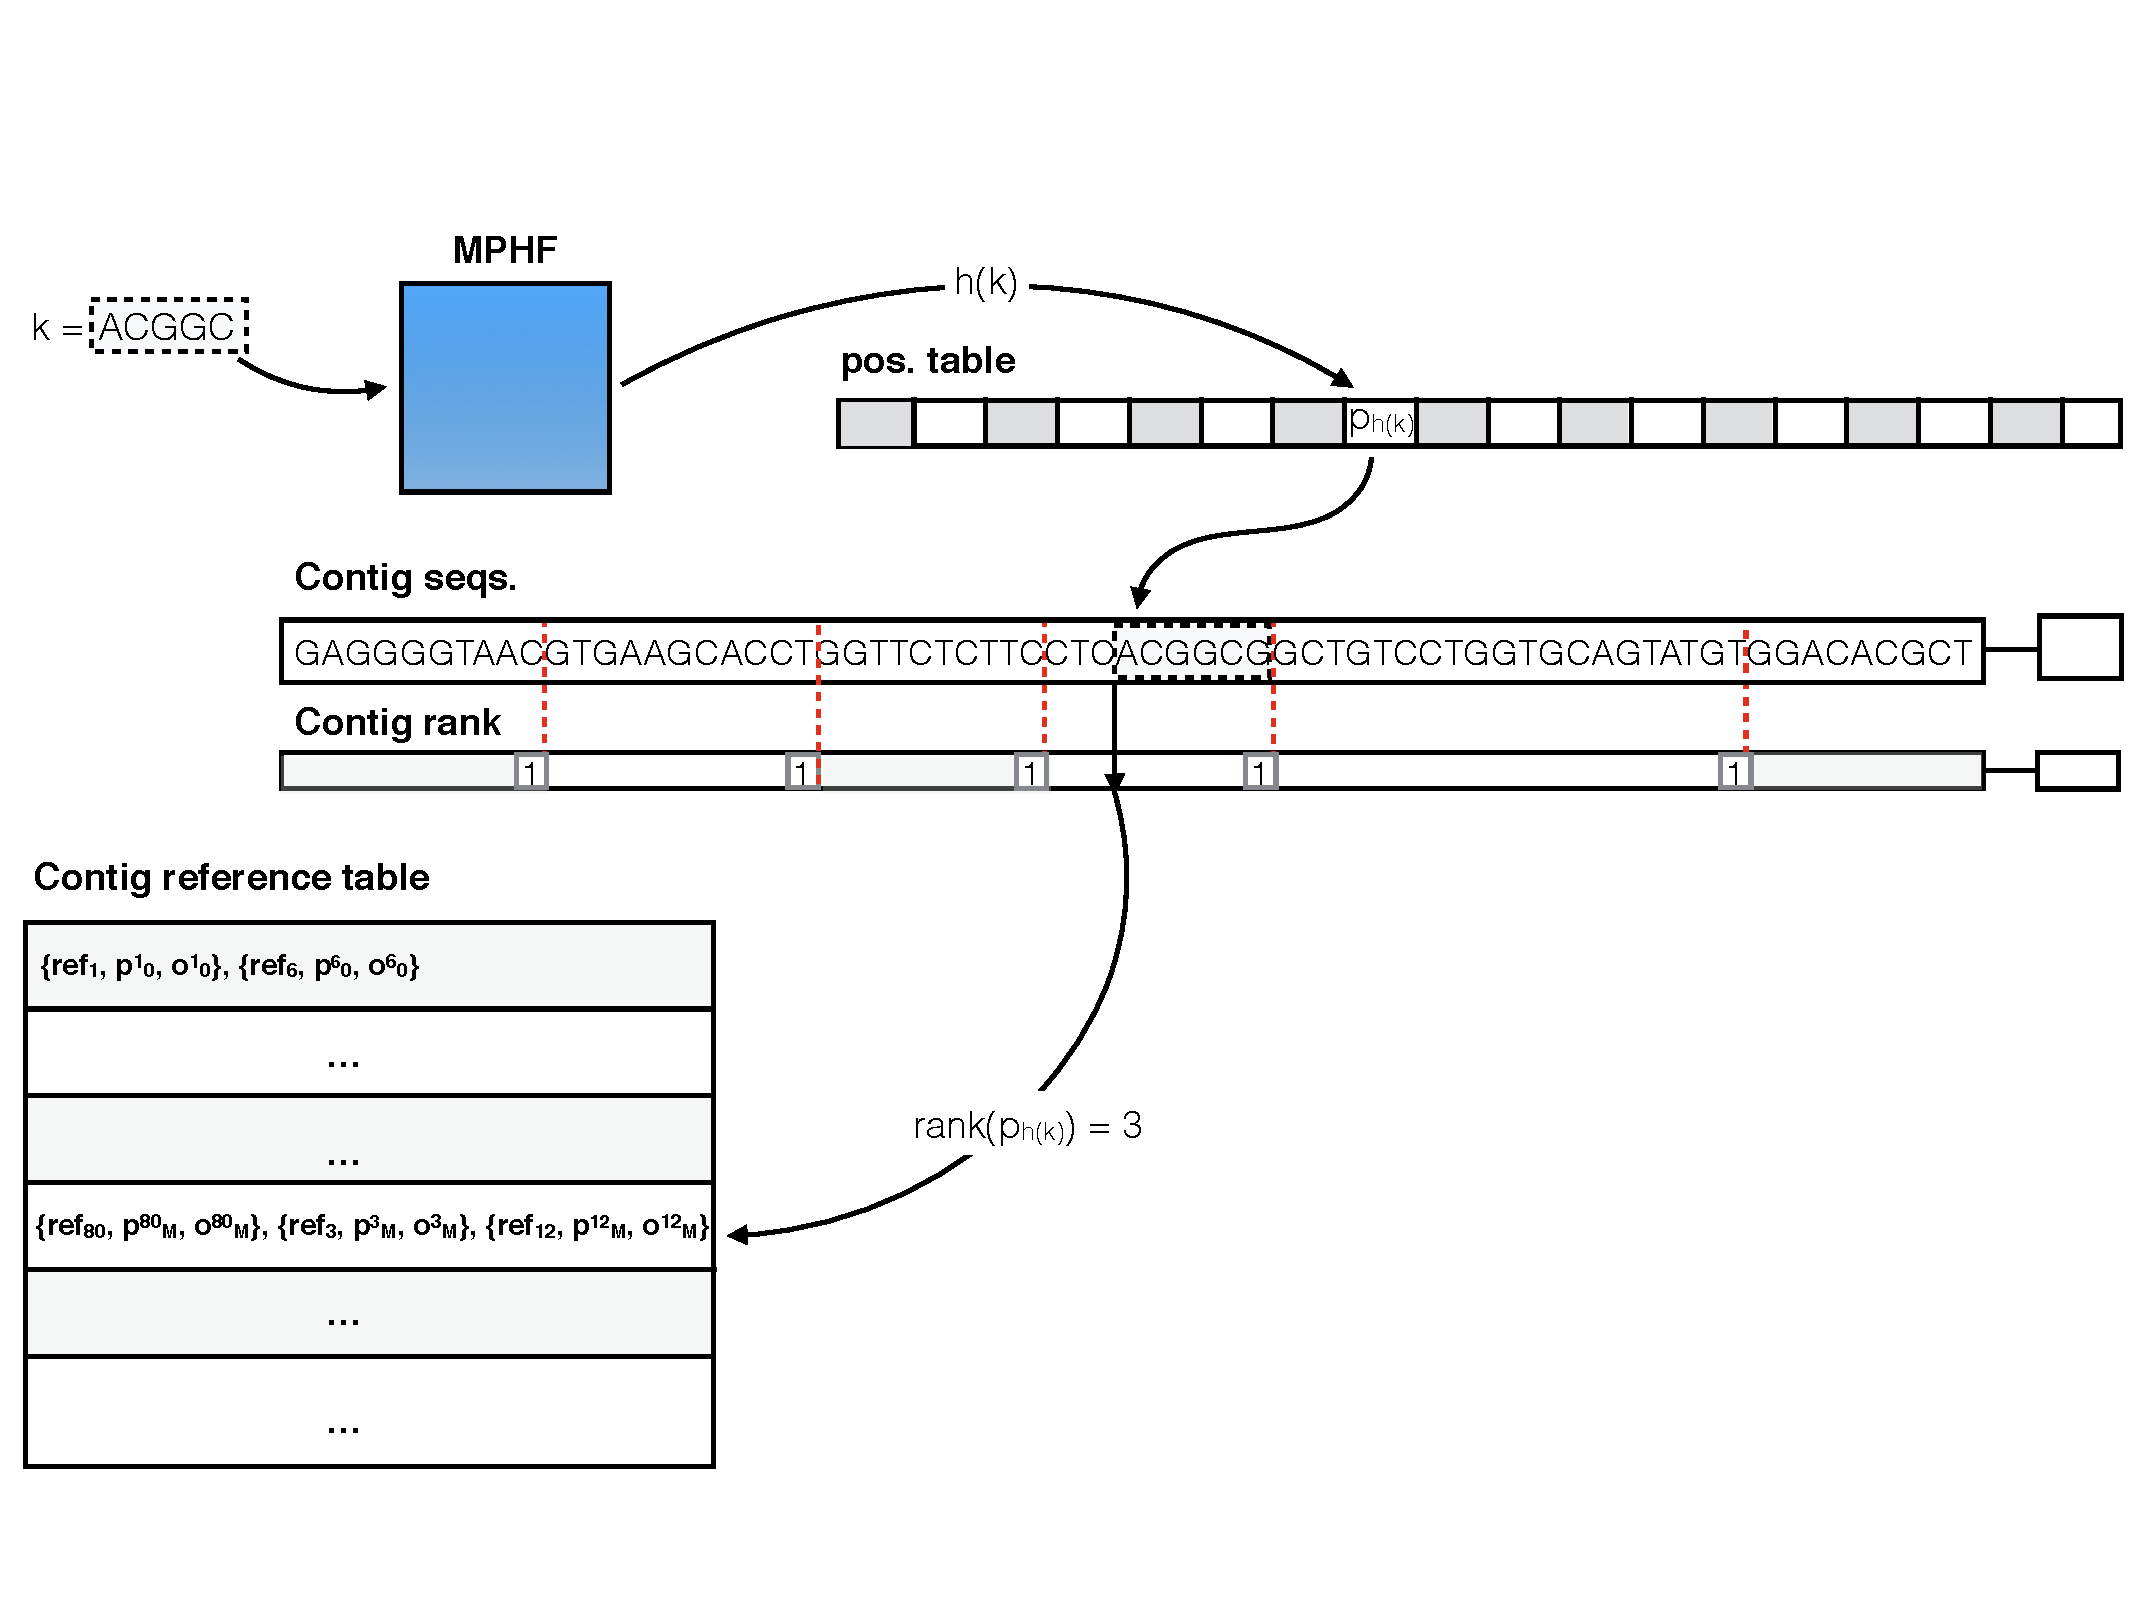
\includegraphics[width=\textwidth]{figs/index_fig}
\caption{An illustration of searching for a particular \kmer in the \emph{dense}
  \pufferfish index. The minimum perfect hash yields the index, $P_{h(x)}$ in the
  \emph{pos} vector where the \kmer appears in the contig array. The \kmer is
  validated against the sequence recorded at this position (and, in this case,
  it matches). A rank operation on $p_{h(x)}$ is performed in the boundary
  vector, which yields the corresponding contig-level information in the contig
  table. If desired, the relative position of the \kmer within the contig can be
  retrieved with an extra select and rank operation.}
\label{fig:dense_index}
\end{figure}


\section{Methods}\label{sec:methods}

We introduce a new data structure, implemented in the software \pufferfish, for
indexing the \ccdbg (and colored variants of it). While we are conscious of
memory usage, we don't aim to build the smallest possible index. Rather, we care
about making the \ccdbg index practical for genomic and metagenomic data while
maintaining very fast query speeds over the index. Here, we introduce both a
\emph{dense} and \emph{sparse} variant of the \pufferfish index, where, as with the
FM-index~\cite{Ferragina2001Experimental}, the sparsity factor can be tuned to
trade off search speed for index size. The sparse index tuned to take maximum space,
is at the same level as dense index regarding space and \kmer query time.

\paragraph*{Pre-processing} We assume as input to \pufferfish, the \ccdbg on the reference
or set of references to be indexed. The \pufferfish software itself accepts as input
a graphical fragment assembly (GFA) format file that describes the \ccdbg.
Specifically, this file encodes the contigs (i.e., non-branching paths) of the
\ccdbg as ``segments'' and the mapping between these contigs and the original
reference sequences as ``paths''. Each path is spelled out with an ordered set of contig IDs and the orientation they are mapped by, so that each contig has an overlap of k-1 with its following contig in the path (either in forward or reverse-complement).
The GFA is an evolving standard that is meant
to be a common format used by tools dealing with graphical representations of
genomes or collections of genomes. We note that there are a number of software
tools for building the \ccdbg directly (i.e., without first building the
un-compacted \dbg). We adopt \twopaco~\cite{minkin2016twopaco}, which employs a
time and memory-efficient, parallel algorithm for directly constructing the
\ccdbg, which can then easily be converted into GFA format. We note that, due to
a technical detail in the way \twopaco constructs the \ccdbg and the GFA file,
this output cannot be used directly, so \pufferfish includes a GFA-to-GFA converter
that prepares the \twopaco-generated GFA file for indexing by
\pufferfish\footnote{Specifically, the \twopaco \ccdbg has two main differences with
  the format that is expected by \pufferfish. First, it is not the case that \kmers
  and their reverse complements will appear only once in the \twopaco \ccdbg.
  Second, the GFA generated by \twopaco assumes that \emph{edges} of size at
  least $k+1$ will act as GFA segments, implying that they will overlap by $k$
  nucleotides. However, we require that segments be of at least size $k$ and
  overlap by exactly $k-1$ nucleotides.}.

\subsection*{The dense \pufferfish index}

Here we describe the basic (i.e., dense) \pufferfish index. The index consists of 6
components, each of which is described below:

\begin{enumerate}

\item The contig sequence array (\cseq) consists of the (2-bit encoded) sequence of all
  contigs of the \ccdbg packed together into a single array. Typically, the size
  of this structure is close to (or smaller than) the size of the 2-bit encoded
  reference sequence, since redundant sequences are represented only once in
  this structure. We note that the contig array contains the sequence of every
  valid \kmer, as well as that of potentially invalid \kmers (those which span
  contig boundaries in the packed array as the contig sequences in the array follow each other without any delimiters or gaps.).
  Therefore, using the next data structure we will set the boundaries of contigs in the array in a way that makes retrieving the borders, knowing position of a contig in the contig array and length of the contig fast in the query process. 
  We denote by $L_s$ the total length (in
  nucleotides) of the contig array.

\item The boundary vector (\bv) is a sparse bit-vector with a length of $L_s$
  bits. The bits of this vector are in one-to-one correspondence with the
  nucleotides of the contig array, and the boundary vector contains a one at
  each nucleotide corresponding to the end of a contig in the contig array, and
  a zero everywhere else. We can retrieve rank of each contig in \cseq using the
  \rank~operation on \bv. $\rank(\bv[i])$ returns number of 1s in \bv before the current index, $i$, or in other words the rank of the current contig. This can be used to get reference information for the current contig from \ctab, the data structure explained in item \ref{items:dense5}.

\item The minimum perfect hash function ($h\left(\right)$) maps every
  \emph{valid} \kmer in the contig array (i.e., all \kmers not spanning contig
  boundaries) to a unique number in $\left[0,N\right)$, where $N$ is the number
    of distinct valid \kmers in \cseq. We make use of the highly-scalable MPHF
    construction algorithm of~\cite{limasset2017fast}.

\item The position vector (\emph{pos}) stores, for each valid \kmer $x$, the
  position where this \kmer occurs in \cseq. Specifically, for \kmer $x$,
  \emph{pos}$\left[h\left(x\right)\right]$ contains the starting position of $x$ in \cseq 
  such that $\cseq\left[h\left(x\right),h\left(x\right) + k\right] = x$.

\item The conitg table \ctab stores, for each contig appearing in \cseq, the reference
  sequences (including reference ID, offset and orientation) where this contig appears in the
  reference. This is similar to a ``posting list'' in traditional inverted
  indices, where all occurrences of the item (in this case, an entire \ccdbg
  contig) are listed. The order of the contigs in the contig table is the same
  as their order in \cseq, allowing the information for a contig to be accessed
  via a simple rank operation on \bv.

\label{items:dense5}

\item \emph{Optionally}, an equivalence class table that records, for each
  contig, the set of reference sequences where this contig appears.
  Pre-computation and storage of these equivalence classes can speed up fast
  mapping approaches (e.g., pseudoalignment).

\end{enumerate}

These structures allow us to index every \kmer in the \ccdbg efficiently, and to
recall, on demand, all of the reference loci where this \kmer occurs. We note
here that the \kmers of the \ccdbg constitute only a subset of the \kmers in
\cseq. We refer to all \kmers in \cseq that do not span the boundary between two
contigs as \emph{valid} \kmers; these are in one-to-one correspondence with the
\kmers of the \ccdbg.

\subsubsection*{\kmer query in the dense \pufferfish index}
By using a MPHF $h$ to index the \emph{valid} \kmers, we avoid the typically
large memory burden associated with standard hashing approaches. Instead, the
identity of the hashed keys is encoded implicitly in \cseq. Given a \kmer $x$, we
can check for its existence and location in the following way. We first compute
$i = h(x)$, the index assigned to \kmer $x$ by $h$. If $i > N$, then we
immediately know that $x$ is not a valid \kmer. Otherwise, we retrieve the
position $p_{i}$ stored in $\texttt{pos}[i]$. Finally, we check if the encoded
string $\cseq[i:i+k]$ is identical to $x$. If so, we have found the
contig location of this \kmer, otherwise, $x$ is not a valid \kmer. 

Given $p_{i}$, we can retrieve the reference positions by computing $r_{p_i} =
\rank(\bv[p_{i}])$, which provides an index into \ctab that is
associated with the appropriate contig. This provides all of the reference
sequences, offsets and orientations where this contig appears. We compute the
offset of \kmer $x$ in the contig as $o_{i} = p_{i} - \select(r_{p_i})$,
in which \select returns the start position of the contig in \ctab.
This allows us to easily project this \kmer's position onto each reference
sequence where it appears. We note that querying a \kmer in the \pufferfish index is
an asymptotically constant-time operation, and that the reference loci for a
\kmer $x$ can be retrieve in $O(\texttt{occ}(x))$ time, where $\texttt{occ}(x)$
is the number of occurrences of $x$ in the reference.

\subsection*{The sparse \pufferfish index}

The \pufferfish index, as described above, is relatively memory-efficient. Yet, what
is typically the biggest component, the \texttt{pos} vector, can still grow rather
large. This is because it occupies $\lg(L_s)$ bits for each of the $N$ valid
\kmers in \cseq. However, at the cost of a slight increase in the practical
(though not asymptotic) complexity of lookup, the size of this structure can be
reduced considerably. To see how, we first make the following observation:

\begin{observation}
  In the \ccdbg (and hence, in \cseq), each valid \kmer occurs exactly once (\kmers occuring between contig boundaries are not considered).
\end{observation}

Hence, any valid \kmer in the \ccdbg is either a complex \kmer (i.e., it has an
in or out degree greater than 1), is a terminal \kmer (i.e., it appears at the
beginning or end of some input reference sequence), or it has a unique
predecessor and successor in the orientation defined by the contig.

We can exploit this observation in \pufferfish to allow \emph{sampling} of the \kmer
positions. That is, rather than storing the position of each \kmer in the contig
array, we store the position only for some subset of \kmers, where the rate of
sampling is defined by a user-defined parameter $s$. For those \kmers that are
not sampled, we store, instead, four pieces of information; the extension that
must be applied to move toward the closest \kmer at a sampled position, whether
or not the corresponding \kmer in \cseq is canonical, whether the extension
to reach the nearest sampled position should be applied by moving to the left or
the right, and a bit vector with the same size as \cseq
that is set to $1$ for any \kmer in \cseq that we've stored its position and $0$
for those that are not sampled.
This idea of sampling the positions for the \kmers is similar to the
idea of sampling the suffix array positions that is employed in the
FM-index~\cite{Ferragina2001Experimental}. This allows us to trade off query
time for index space, to allow the \pufferfish index to scale to large genomes or
collections of genomes. 


\subsubsection*{\kmer query in the sparse \pufferfish index}  \kmer query in the sparse \pufferfish index
is the same as that in the dense index, except for the first step ---
determining the position of the \kmer $x$ in \cseq. When we query the MPHF with
$x$ to obtain $i = h(x)$, there are three possible results. 
\begin{enumerate}
\item In the first case,
we could have that $i \geq N$, implying, just as in the dense case, that $x$ is
not a valid \kmer. 
\item Second, we could have that $\texttt{sampled}[i] = 1$,
implying that we have explicitly stored the position for the $i$-th \kmer, in
which case we can retrieve that position as $p_{i} = \texttt{pos}[\texttt{rank}(\texttt{sampled}[i])]$ and
proceed as before in the dense case to validate $x$ and retrieve its reference positions.
\item The third case is that $i < N$ and $\texttt{sampled}[i] = 0$. In this case, we do not know
the position where $x$ would occur in \cseq, and we must find the closest sampled position.
This is done with algorithm \ref{alg:nextSample}
\end{enumerate}

\begin{algorithm}
\caption{Find Next Sample}\label{alg:nextSample}
\begin{algorithmic}[1]
\Procedure{FindNextSample}{}
\State $\textit{e} \gets \textit{extension} \text{ size}$
\State $X \gets \textit{\kmer}$
\State $EV \gets \text{extension vector}$

\State $i \gets \textit{MPHF(\kmer)}$
\State $X_{rc} \gets \textit{reverseComplement}(X)$
%\BState \emph{loop}:
\While{\textbf{not} $isSampled[i]$} 

%\If {$isSampled[i]$}
%\State \textbf{goto} \emph{end}.
%\EndIf
\State $extIdx \gets i-rank(isSampled[i])$
\If {$isCanonical[i]$ \textbf{and} $isDirectionRight[i]$}
\State $X \gets X[e:] + EV[extIdx]$.
\EndIf
\If {\textbf{not} $isCanonical[i]$ \textbf{and} $isDirectionRight[i]$}
\State $X \gets X_{rc}[e:] + EV[extIdx]$.
\EndIf
\If {$isCanonical[i]$ \textbf{and} \textbf{not} $isDirectionRight[i]$}
\State $X \gets EV[extIdx] + X[:-e]$.
\EndIf
\If {\textbf{not} $isCanonical[i]$ \textbf{and} \textbf{not} $isDirectionRight[i]$}
\State $X \gets EV[extIdx] + X_{rc}[:-e]$.
\EndIf
\State $i \gets \textit{MPHF(\kmer)}$
\State $X_{rc} \gets \textit{reverseComplement}(X)$
\EndWhile
%\BState \emph{end}:
\Return $X$
\EndProcedure
\end{algorithmic}
\end{algorithm}


Intuitively, algorithm \ref{alg:nextSample} appends nucleotides stored in the
\texttt{extension} array to $x$ to generate a new \kmer, $x'$ which either has a
sampled position, or is closer to a sampled position than is $x$. The extension
process is repeated with $x'$, $x''$, etc. until a sampled position is reached.
At that point, one simply traverses back to the position in \cseq implied by the
sampled position and sequence of extension operations, for the original \kmer
$x$. The rest of the search proceeds as for the dense case. The whole process of
\kmer query in sparse index is illustrated in Fig \ref{fig:sparse_query} through an example.

\begin{figure}
  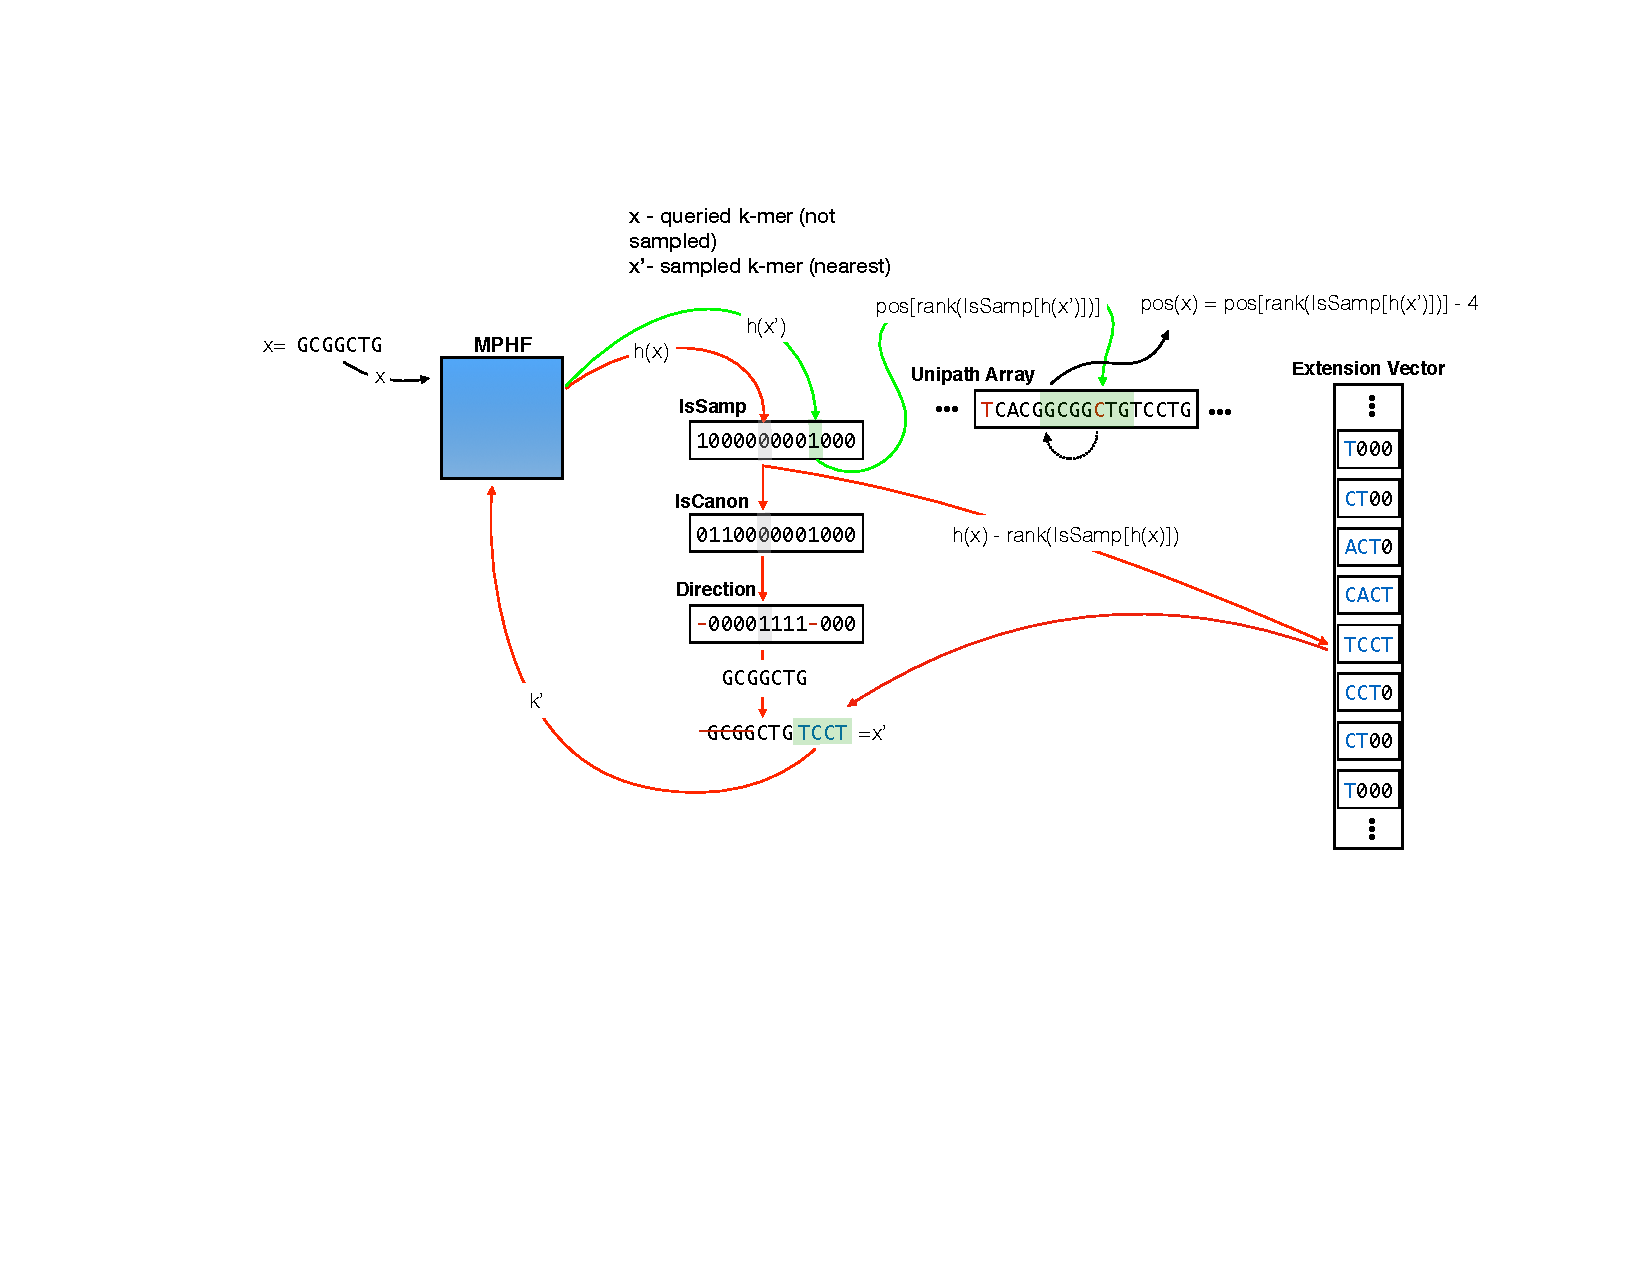
\includegraphics[width=\textwidth]{figs/query_sparse}
\caption{An illustration of searching for a particular \kmer in the \emph{sparse}
  \pufferfish index with sample factor ($s$) of 9 and extension size ($e$) of 4.
  All vectors \emph{isSampled}, \emph{isCanon}, and \emph{ExtRight} have the same
  size which is equal to length of the total number of valid \kmers.
  The minimum perfect hash yields the index, $h(x)$ for $x=CAGCCGC$ in the
  \emph{isSampled} vector where we'll find out that the \kmer is not sampled.
  \emph{isCanon} being $0$ at the same index as $h(x)$ shows that the \kmer
  is not canonical. Since we keep the extensions in canonical format we need to 
  canonicalize the \kmer to $x'=GCGGCTG$ first. Then based on the value of 
  $\text{\emph{ExtRight}}_{h(x)}$, we know that to get to the closest sampled \kmer
  we need to append the extension to the right of the current \kmer.
  The extension is extracted from \emph{QueryExt} vector. Considering the fact
  that we just keep the extensions for \kmers that are not sampled,
  to find the index of the current \kmer's extension we need to
  subtract the index of the \kmer by total number
  of \kmers that have been sampled up to this position which is equal to 
  total number of $1$s in \emph{isSampled} vector before $h(x)$ for which we use the
  \emph{rank} operation. Therefore, the extension index will be $h(x)-rank(isSampled[h(x)])$.
  We create the new \kmer $x'$ by cropping the first four bases off the current \kmer and
  appending the new extension to its right and repeat the same process for the new \kmer.
  This time, the \kmer is sampled and hence, we go directly to the index in the \emph{UnipathArray}
  that the \emph{sampledPos} vector points us to. To check if the original \kmer we searched for
  exists, we need to compare the \kmer starting from $4$ bases before the current position 
  with the canonic of original \kmer $x=CAGCCGC$ since we just appended one extension of size 4
  to the end of this \kmer. Generally speaking, we need to revert all the extension appendings 
  by walking over the \emph{UnipathArray} vector to the left and right with the same steps as
  extension size until we stop at the right position that we expect the \kmer at that position to be the
  same as the one we searched.}
\label{fig:sparse_query}
\end{figure}



By altering the stored extension size $e$ and the maximum sampling rate $s$, one
can limit the maximum number of extension steps (and hence the maximum number of
hash lookups) that must be performed in order to retrieve the potential index of
$x$ in \cseq. A denser sampling and longer extensions require fewer possible
extension steps, while a sparser sampling and shorter extensions require less space
for each non-sampled position. If $e \geq \frac{s}{2}$, one can guarantee that
at most a single extension step needs to be performed for any \kmer query, which
allows \kmer queries to remain, practically very fast while still considerably
reducing the index size for large reference sequences.

Even though the sparse index maintains a number of extra bit vectors not maintained
in the dense index, it is still usually considerably smaller.
Assume a case where the extension length $e$ is half of the sampling factor $s$.
Since we keep the extension required to get to 
the closest position in left or right direction, we would need to keep
$\frac{s}{2}$ bases for a kmer with each base represented in 2 bits, which corresponds to 
$\frac{s}{2}\times 2 = s$ bits per \kmer for the extension vector. Therefore, if we put all the new 
vectors of extension, canonical, direction, and isSampled together it'll be $s+1+1+1=s+3$ bits 
per each non-sampled \kmer compared to $\lg(L_s)$ bits that we had to keep in 
\emph{pos} vector. Therefore, as long as $[s+3< \lg(L_s)]$ we save space by sparse indexing.
In a typical data set such as human genome with $\lg(L_s) \sim= \lg(3B) \geq 30$ bits, by choosing
$s=9$ which means we'll sample each 9th \kmer, we will save $\sim18$ bits per each non-sampled \kmer.
%\todo{put actual numbers}

\section{Results}\label{sec:results}

We explored the memory and time requirements for building a text index using
\pufferfish and two other tools, \bwa and \kallisto. We also benchmark the speed of
\kmer lookup (the fundamental building block of \bwa's alignment and \kallisto's
pesudoalignment) under these different data structures. We performed these
benchmarks on a number of different reference sequences, selected to show how
the different indexes scale as the underlying reference size and complexity
increase. \bwa and \kallisto both have the complete package for
indexing a data set. For \pufferfish however, we first need to build the \ccdbg using the available
tools. We build the \ccdbg and dump it in GFA format using \twopaco. Then, as the output does
not satisfy our definition of a compacted dbg, we need to have another preparation 
step to convert the GFA file. We call this process\emph{pufferization}, and it converts the GFA file to the format accepted by pufferfish
(each \kmer should be appear only once through out all the unitigs and unitigs should have an overlap of $k-1$ bases).
Then we will build both dense and sparse index and benchmark the time and memory for all these steps of the pipeline individually.
Final comparison between the time and memory that pufferfish requires versus the other tools should be the aggregated time and
maximum memory of the whole pufferfish pipeline.
All experiments
were performed on an Intel(R) Xeon(R) CPU (E5-2699 v4 @2.20GHz with 44 cores and
56MB L3 cache) with 512GB RAM and a 4TB TOSHIBA MG03ACA4 ATA HDD running ubuntu
16.10, and were carried out using a single thread except for cdBg building step using TwoPaCo.

%\todo{explain datasets}

\begin{table}
\begin{center}
\begin{tabular} {| l || c c c| c c c|}
\hline
\multirow{2}{*}{Indexing Tools} & \multicolumn{3}{c|}{Memory (MB)} & \multicolumn{3}{c|}{Time (secs)} \\
\cline{2-7}
& \parbox[c]{2.5cm}{Human\vfill Transcriptome} & 
\parbox[c]{1.5cm}{Human\vfill Genome} & 
\parbox[c]{1.5cm}{Bacterial \vfill Genome} & 
\parbox[c]{2.5cm}{Human \vfill Transcriptome} & 
\parbox[c]{1.5cm}{Human \vfill Genome} & 
\parbox[c]{1.5cm}{Bacterial \vfill Genome} \\
\hline
 
\bwa & 292 & 4,443 & 32,213 & 2:56 & 0:58:27 & 13:11:45\\
\hline
\kallisto & 3,552 & 150,657 & NA & 3:05 & 3:27:42 & >2 days\\
\hline
\twopaco & 1,466 & 18,004 & NA & 2:47 & 0:56:12 & >2 days \\
pufferize & 584 & 27,438 & 49,510 & 0:10 & 0:21:53 & 54:11\\
pufferfish dense & 438 &  20,000 & 30,224 & 1:16 & 0:51:20 & 1:27:08 \\
pufferfish sparse & 331 & 17,745 & 29,811 & 1:44 & 1:10:48 & 2:02:34\\
\hline
\end{tabular}
\caption{
  Construction time and memory for \pufferfish, \kallisto, and \bwa for different
  datasets. 
}
\vspace{-2.5em}
\label{tab:construction}
\end{center}
\end{table}

\begin{table}
\begin{center}
\begin{tabular} {| l || c c c| c c c|}
\hline
\multirow{2}{*}{Indexing Tools} & \multicolumn{3}{c|}{Memory (MB)} & \multicolumn{3}{c|}{Time (secs)} \\
\cline{2-7}
& \parbox[c]{2.5cm}{Human\vfill Transcriptome} & 
\parbox[c]{1.5cm}{Human\vfill Genome} & 
\parbox[c]{1.5cm}{Bacterial \vfill Genome} & 
\parbox[c]{2.5cm}{Human \vfill Transcriptome} & 
\parbox[c]{1.5cm}{Human \vfill Genome} & 
\parbox[c]{1.5cm}{Bacterial \vfill Genome} \\
\hline
 
         
  
\bwa & 308 & 4,440 & 33,333 & 1:09:14 & 1:11:29 & 6:41\\
\hline
\kallisto & 3,337 & 110,646 & 120,748 & 6:17 & 24:29 & 20:06\\
\hline
pufferfish dense & 500 & 17,661 & 28,596 & 6:05 & 16:14 & 3:34 \\
pufferfish sparse & 315 & 12,510 & 20,470 & 17:41 & 26:38 & 4:26\\
\hline
\end{tabular}
\caption{
  \kmer lookup time and memory for \pufferfish, \kallisto, and \bwa for different
  datasets. 
}
\vspace{-2.5em}
\label{tab:query}
\end{center}
\end{table}

As expected we see in table \ref{tab:construction} that \pufferfish takes longer to build the index compared to a linear indexing based
tool such as \bwa and stands almost in the same level as \kallisto which is another graph-based indexing tool. 
However, the amount of memory it needs is considerably smaller than \kallisto, so that for a large reference
such as the human genome, it consumes $\sim6$ times less memory. Comparing the \kmer lookup time in table \ref{tab:query}, 
we can see how using a graph-based indexing system can outperform \bwa regarding time and still because of the succinct
data structures used in the index building and the compression algorithms used in that would need almost the same memory as \bwa
which is much less than what \kallisto needs to load all the indexing data structure.
The disk space and memory \pufferfish needs are very similar, unlike \kallisto, where the hash table consumes
much more RAM than what serialized version requires on disk.

\begin{table}
\begin{center}
\begin{tabular} {| l || c c c |}
\hline
\parbox[c]{2cm}{Indexing \vfill Tools} & 
\parbox[c]{2.5cm}{Human\vfill Transcriptome} & 
\parbox[c]{1.5cm}{Human\vfill Genome} & 
\parbox[c]{1.5cm}{Bacterial \vfill Genome}  \\
\hline   
       
\bwa & 347M & 5.12G & 37.8G \\
\hline
\kallisto & 1.7G & 58G & 87G \\
\hline
pufferfish dense & 387M & 16G & 26G \\
pufferfish sparse & 271M & 11G & 18G \\
\hline
\end{tabular}
\caption{
  Disk space each of \pufferfish, \kallisto, and \bwa will take for different
  datasets. 
}
\vspace{-2.5em}
\label{tab:disk-space}
\end{center}
\end{table}
%kallisto construction on GRCh38 (primary)
%%
%rob@newton:~ /usr/bin/time ~/kallistokmerlookup/build/src/kallisto index -k 31 -i GRCh38.primary\_assembly.genome.fixed.kalidx GRCh38.primary\_assembly.genome.fixed.fa
%
%[build] loading fasta file GRCh38.primary\_assembly.genome.fixed.fa
%[build] k-mer length: 31
%[build] counting k-mers ... done.
%[build] building target de Bruijn graph ...  done
%[build] creating equivalence classes ...  done
%[build] target de Bruijn graph has 38967126 contigs and contains 2652229049 k-mers
%
%7911.72user 1873.99system 2:45:24elapsed 98\%CPU (0avgtext+0avgdata 154270332maxresident)k
%0inputs+119758728outputs (0major+3389704442minor)pagefaults 0swaps
%%

We note that on large sequences (e.g., the human genome)
kallisto seems to require an inordinate amount of time (i.e., days) to load the index into memory. This appears to
occur during the final phase of index loading. However, we were able to resolve this issue and hence
provide \kmer query times for these samples (otherwise just amortizing the index loading time over each \kmer would result
in lookup times tens of thousands of times slower than the other tools).

\section{Conclusion and Future Work}
In this chapter we proposed a new efficient data structure for indexing compacted de Bruijn graphs and also its implementation in a tool called \pufferfish. We showed how \pufferfish can achieve a balance between time and space resources. By building upon a MPHF~\cite{limasset2017fast}, we provide practically fast \kmer lookup, and by carefully organizing our data structure and making use of succinct representations where applicable, we greatly reduce the space compared to traditional hashing-based implementations. The main components of the data structures are a minimum perfect hash function (MPHF) built on \kmers, the concatenated unitig array from which the \kmers are sampled, a bit vector that marks the boundary of unitigs in the concatenated array, a vector containing the offset position for the \kmers, and a unitig table enumerating the occurrences of each unitig in the reference sequence.

Moreover, we presented two variants of the \pufferfish data structure; namely, a dense and a sparse variant. The first is optimized for fast queries and the second provides the user with the ability to trade off space for speed in a fine-grained manner. In the sparse index, we only keep offset positions for a subset of \kmers. To query an unsampled \kmer, the sparse representation is aided with a few auxiliary data structures of much smaller size. Since the largest component of the index is the position vector, adopting this sparse representation significantly reduces the required memory and disk space. Our analyses suggest that pufferfish (dense) achieves similar speed to existing hash-based approaches, while greatly reducing the memory and disk space required for indexing. We consider indexing and query on both small (human transcriptome) and large (~8000 bacterial genomes) reference datasets. Pufferfish strikes a desirable balance between speed and space usage, and allows for fast search on large reference sequences, using moderate memory resources. 

Having built an index for a reference genome or transcriptome using \pufferfish, the immediate future work would be implementing the applications of such an index. These applications fall into the categories that need mapping or alignment as their initial step. Therefore, we would like to adopt an existing aligner or mapper such as RapMap~\cite{srivastava2016rapmap} or Selective Alignement~\cite{sarkar2017towards} and modify it to use \pufferfish as its indexing methodology. Later we can use the result of this aligner for RNA-sequence quantification, metagenomic abundance estimation, or population-level read tasks. We expect the memory efficiency of \pufferfish indexing will be beneficial in working with larger collections of genomic and transcriptomic data sets. Moreover, by indexing the genome and transcriptome together using \pufferfish, we can discover novel exon splicing. 
%Genome comparison and structural variant detection in a group of genomes can also be one of the immediate results of the \pufferfish as construction and query time are both reasonably fast and also memory-efficient.


\chapter{Conclusion, Discussion, and Future Work}

When working at the scale of whole genomes, the problem of extending indexing strategies to graphs becomes very important. In addition to that, indexing more than one sample in the same data structure adds to the complexity of the problem. In this document, we presented two data structures for indexing collection of genomes, transcriptomes, or sample reads on top of colored de Bruijn graphs and compacted de Bruijn graphs. Both of these data structures make use of succinct representations along with rank and select operations. As the future direction, we are interested in exploring different applications for these two data structures and also investigating the relationship between them to see how we can merge these two into one multi-purpose data structure that can be part of different pipelines of mapping and assembly and merged with different representations of de Bruijn graph including succinct representations like BOSS and compacted de Bruijn graph.

In colored de Bruijn graph, the only information we keep per each \kmer in the indexing data structure regarding different samples (genomes, sequence read samples, etc.) is just its membership. Therefore, one future direction for indexing a colored de bruijn graph can be having different types of annotations in one compacted package in addition to just membership; annotations like position and orientation for a referenced base colored de Bruijn graph and frequency for both referenced based and assembly cases.
Moreover, it will be interesting to explore how multiple attributes could be efficiently stored simultaneously, and how potential correlations between these attributes might be exploited. For example, there may be natural extensions of similar coding schemes to the compacted de Bruijn graph, where one might also be able to take advantage of the coherence in annotation (i.e., color or count information) shared among the constituent \kmers of a contig, allowing one to store only the information where these annotations change during traversal.

Another area of interest toward improving space of colored de Bruijn graphs can be exploring other ways to use fewer colors to represent all samples instead of compressing the final color matrix. One of the approaches is to reuse the previously assigned colors in disjoint subgraphs or even non-adjacent edges. In other words, we cannot reuse the same color for a different sample for \kmers that are adjacent, but we can have colors that are globally reused. In this case we need to have a proper mapping from a color to its corresponding samples in different disjoint areas of the graph. As a de Bruijn graph is a special type of directed graphs with each node having at most $4$ incoming and $4$ outgoing edges, the chromatic number of such graph is at most $9$ (maximum degree + 1). Therefore, if we can design an efficient color-to-sample mapping, we can reduce size of the graph by not assigning one bit to each color. In this case, we are approaching the problem from a different direction than compressing the color matrix that we explained in \ref{sec:rainbowfish}.

The main advantage of a data structure like \pufferfish compared to a linear index is the ability of efficiently mapping reads to a population of genomes or individual genomes with annotated variants. Current tools that are used for alignment and mapping are either suitable for genome or transcriptome, but not both. \pufferfish fills the gap by allowing fast and accurate mapping to a collection of genomes and transcriptomes at the same time. This ability paves the way for accomplishing applications such as ``novel exon discovery" or ``RNA-seq quality control''. 
Because of the distinction between methods that map to transcriptome and those that map to genome, we lose the information that can be derived by puting both of these mappings together. One immediate outcome of having short reads mapped to both genome and transcriptome is in ``RNA-seq quality control''. If we just look at the transcriptome mapping outcome, we would just simply throw all the non-mapped reads out, ignoring the fact that not being mapped at all is a different observation than being mapped to an intron. A large fraction of reads mapping to introns is an evidence that the RNA-seq experiment failed to provide the required quality. Having reads mapped to both genome and transcriptome, we can account for such experiments' failure. Another application of dual mapping which is of a biological importance is looking for any intron retention in an RNA-seq read set. High probability of retaining introns in reads from RNA-seq experiments is known to be associated with certain desease phynotypes. By mapping the reads to just transcriptomes, we can never be aware of any intron retentions.

Another problem that can be answered using \pufferfish is finding ``structureal variations'' in a metagenomic data set or accross different samples of the same individual. One particular way to approach this problem is through genome alignment. Having a genome indexed using \pufferfish, we can map another genome to it instead of a set of short reads. In a different view, we can index multiple genomes at the same time into one data structure combining the concepts of indexing a colored de Bruijn graph and a compacted de Bruijn graph. There are a lot of small scale variations happening across two genomes that can be the result of an error in read sequencing process or not informative enough. However, the biologically interesting variations across genomes are those that happen in scales longer than the length of the read. Building \pufferfish along a collection of genomes will allow us to search for such variations. One specific type of variation can be inversions happening alongside of the genome, so that we have a one to one correspondance between \kmers of two genomes and at some location the positions start decreasing in one genome as we increase position in the other. The inversions can be identified by a data structure like \pufferfish that keeps position of a \kmer in all the references.




\bibliography{introduction,merged}
%\input{bibliography}

\end{document}